\documentclass[12pt]{article}

\usepackage[UTF8]{ctex}
\usepackage{appendix}
\usepackage{enumerate}
\usepackage{amsmath}
\usepackage{graphicx}
\usepackage{cite}
\usepackage{ listings} 
\usepackage{bigstrut}
\usepackage{multirow}
\usepackage{geometry}
\usepackage{longtable}
\usepackage{listings}
\usepackage{color}
\usepackage{xcolor}
\usepackage[section]{placeins}
\usepackage[colorlinks,linkcolor=blue]{hyperref}
\usepackage[]{caption2} 
\renewcommand{\captionlabeldelim}{ }
\usepackage{titlesec}  
\usepackage{titletoc}
\geometry{a4paper,scale=0.8}
\renewcommand\figurename{\heiti\zihao{5} 图}
\renewcommand\tablename{\heiti\zihao{5} 表}
\renewcommand{\contentsname}{\centering 目录}
\lstset{
breaklines,
    columns=fixed,       
    numbers=left,                                        % 在左侧显示行号
    frame=none,                                          % 不显示背景边框
    backgroundcolor=\color[RGB]{245,245,244},            % 设定背景颜色
    keywordstyle=\color[RGB]{40,40,255}\bf,                 % 设定关键字颜色
    numberstyle=\footnotesize\color{darkgray},           % 设定行号格式
    commentstyle=\it\color[RGB]{0,96,96},                % 设置代码注释的格式
    stringstyle=\rmfamily\slshape\color[RGB]{128,0,0}\small,   % 设置字符串格式
%labelstyle=\tiny\color[RGB]{255,0,0},
    showstringspaces=false,                              % 不显示字符串中的空格
    escapeinside=``,
    language=VHDL,                                        % 设置语言
}
\begin{document}%文档从这里开始。
\begin{center}
\renewcommand\refname{参考文献}

\renewcommand\appendix{\setcounter{secnumdepth}{0}}
\begin{figure}[h]
\centering
  
\includegraphics[width=.6\textwidth]{image001.png} 
\end{figure}
\thispagestyle{empty}
\songti\zihao{0}\textbf{EDA设计(II)}\\ 
\zihao{1}\ \\ \textbf{多功能数字时钟}\\\ \\\ 
\zihao{3}
\renewcommand\arraystretch{1.5}
\begin{tabular}{p{1.7cm}p{0.2cm}p{3.5cm}p{1.7cm}p{0.2cm}p{3.5cm}}
作\ \  者&\textbf{:}&\ \ \ \ 许晓明&学\  \ 号&\textbf{:}&9161040G0734\\\cline{3-3}\cline{6-6}
学\  \ 院&\textbf{:}&\multicolumn{4}{c}{电子工程与光电技术学院}\\\cline{3-6}
专\ \ 业&\textbf{:}&\multicolumn{4}{c}{电子信息工程}\\\cline{3-6}
班\ \ 级&\textbf{:}&\multicolumn{4}{c}{9161042103}\\\cline{3-6}
题 \ \ 目&\textbf{:}&\multicolumn{4}{c}{EDA设计(II):}\\\cline{3-6}
&&\multicolumn{4}{c}{多功能数字钟设计}\\\cline{3-6}
指导者&\textbf{:}&\multicolumn{4}{c}{谭雪琴}\\\cline{3-6}
\end{tabular}\\
\ \\
\ \\
\ \\
\ \\
2018\ 年\ 12月
\end{center}
\newpage
\ 
\thispagestyle{empty}
\newpage
\thispagestyle{empty}
\zihao{4}
\newpage
\thispagestyle{empty}
\begin{center}\textbf{摘要}\end{center}
\par
数字钟是用数字电路技术实现计时的钟表。与机械钟相比,其准确性与直观性更高,使用寿命也更长。本文基于 QuartusⅡ软件,通过实物电路与 VHDL 语言编程结合的方式实现数字钟,其具有 24 小时计时,时钟星期、时、分、秒快速校对,时钟保持、清零,整点报时,铃声,万年历等功能。\par
本文采用了自顶向下的模块式分析设计方法,首先分析了多功能数字钟的设计要求及所需实现的功能,将整个电路分为分频模块,校时模块,清零保持模块,计时模块,音乐模块,显示模块,万年历模块等。\par在具体设计时,采用的是自底向上的设计方法。即首先设计各种基础模块,然后设计功能模块,最后再进行综合设计。在设计同时,对每个模块所需要的功能进行仿真验证或直接下载到实验平台进行验证。在验证了功能的正确性后,连接各个模块组成一个总的电路。最后对总的电路分配好引脚,下载到实验板上。\par实验的最终结果,在满足基本功能的情况下进行了创新,达到了不错的效果。\par
本报告首先分析了数字时钟的工作原理,并解释说明各子模块的设计原理及调试过程。其次对实验最终结果进行总结。在报告的最后总结了实验过程中出现的问题困难以及相应的解决方法。\newline\newline
\textbf{关键词:}QuartusII \ 多功能数字时钟\ 
万年历\ 
模块设计\ 
仿真
\newpage
\thispagestyle{empty}
\begin{center}\textbf{Abstract}\end{center}\par
The digital clock is a timepiece that uses digital circuit technology to achieve timing. Compared with mechanical clocks, it is more accurate and intuitive, and has a longer service life. Based on Quartus II software, this paper realizes the digital clock through the combination of physical circuit and VHDL language programming. It has 24-hour timing, fast calibration of clock week, hour, minute and second, clock hold, clear, hourly chime, ringtone, perpetual calendar, etc. Features.

This paper adopts the top-down modular analysis design method. Firstly, it analyzes the design requirements of the multi-function digital clock and the functions that need to be realized. The whole circuit is divided into frequency division module, calibration module, zero-keeping module, timing. Module, music module, display module, perpetual calendar module, etc.

In the specific design, the bottom-up design method is adopted. That is, first design various basic modules, then design functional modules, and finally carry out comprehensive design. At the same time of design, the functions required for each module are simulated or directly downloaded to the experimental platform for verification. After verifying the correctness of the function, connect each module to form a total circuit. Finally, the pins are allocated to the total circuit and downloaded to the experiment board.

The final result of the experiment was innovated with basic functions and achieved good results.

This report first analyzes the working principle of the digital clock and explains the design principle and debugging process of each sub-module. Secondly, the final results of the experiment are summarized. At the end of the report, the problems encountered during the experiment and the corresponding solutions were summarized.\newline\newline
\textbf{key words:}QuartusII,Multifunction digital clock,
Perpetual calendar,
Module design,
simulation
\newpage

\tableofcontents
\thispagestyle{empty}
\newpage
\thispagestyle{empty}
%\zihao{5}
\setcounter{page}{1}
\section{设计要求说明}
利用QuartusII软件设计一个数字计时器,可以完成00:00:00到
23:59:59的计时功能,并在控制电路的作用
下具有保持、清零、快速校时、快速校分、
整点报时等功能。并下载
到SmartSOPC实验系统中。
\subsection{设计基本要求}
时钟的基本设计具体要求如下:
\begin{enumerate}[1、]
\item 能进行正常的时、分、秒计时功能;
\item 分别由六个数码管显示时分秒的计时;
\item $K_1$是系统的使能开关($K_1=0$正常工作,$K_1=1$时钟
保持不变);
\item $K_2$是系统的清零开关($K_2=0$正常工作,$K_2=1$时钟
的分、秒全清零);
\item $K_3$是系统的校分开关($K_3=0$正常工作,$K_3=1$时可
以快速校分);
\item $K_4$是系统的校时开关($K_4=0$正常工作,$K_4=1$时可
以快速校时);
\item 使时钟具有整点报时功能(当时钟计到59’53”时开始报时,在59’53”, 59’55”,59’57” 时报时频率为512Hz,59’59”时报时频率为1KHz)。
\end{enumerate}
\subsection{设计提高部分要求}
完成基本设计要求后,可选做提高性要求。实验中我做的功能有:
\begin{enumerate}[1、]
\item 星期计时功能;
\item 铃声功能;
\item 万年历功能。
\end{enumerate}
\section{方案论证(整体电路的工作原理)}
按功能,时钟可以分为以下几个模块:分频模块、计时模块、清零保持模块、校时模块、音乐模块、显示模块、万年历模块等。其中,需要用到开关的部分都需要加消颤功能。根据各模块功能的要求,各大模块又可以分成几个小的基本模块,模块间联系大致如图\ref{fig:lianxi}。\par
\begin{figure}[htbp]%%图
	\centering  %插入的图片居中表示
	\includegraphics[width=\textwidth]{picture/all.png}  %插入的图,包括JPG,PNG,PDF,EPS等,放在源文件目录下
	\caption{各模块间联系}  %图片的名称
	\label{fig:lianxi}   %标签,用作引用
\end{figure}
首先由分频模块产生脉冲信号,输入到基本计时模块中,计时模块的时、分、秒和星期等各位信号均输出到显示模块中,而计时电路的分位和秒位信号也输出到报时模块中,而清零、保持模块,校时模块都是在此基础上对基本计时模块的控制。万年历模块则是在基本模块上的附加模块。
\section{各子模块设计原理}

\subsection{分频模块}
分频模块实现的功能是将实验箱提供的48MHZ的高频信号变成所需的1Hz、2Hz、500Hz和1kHz的信号,其中,1kHz 用于报时最后一声,500Hz 用于报时的前几声,2Hz 用于校时,1Hz 用于计时。

\subsubsection{2分频}
借助D触发器实现二分频,原理图见图\ref{fig:2fenpin},仿真波形见图\ref{fig:fangzhen2fenpin},封装图见图\ref{fig:fengzhuang2fenpin}。
\begin{figure}[hp]
	\centering  
	\includegraphics[width=\textwidth]{picture/2fenpin.png} 
	\caption{}
	\label{fig:2fenpin}   
\end{figure}
\begin{figure}[hp]
	\centering  
	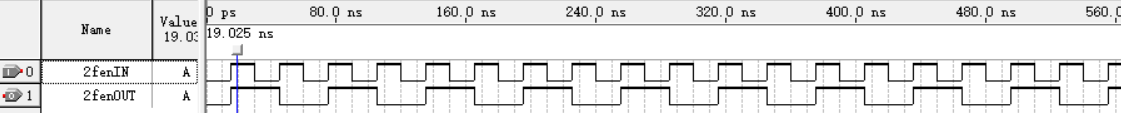
\includegraphics[width=\textwidth]{picture/TIM20181210152648.png} 
	\caption{}
	\label{fig:fangzhen2fenpin}   
\end{figure}
\begin{figure}[hp]
	\centering  
	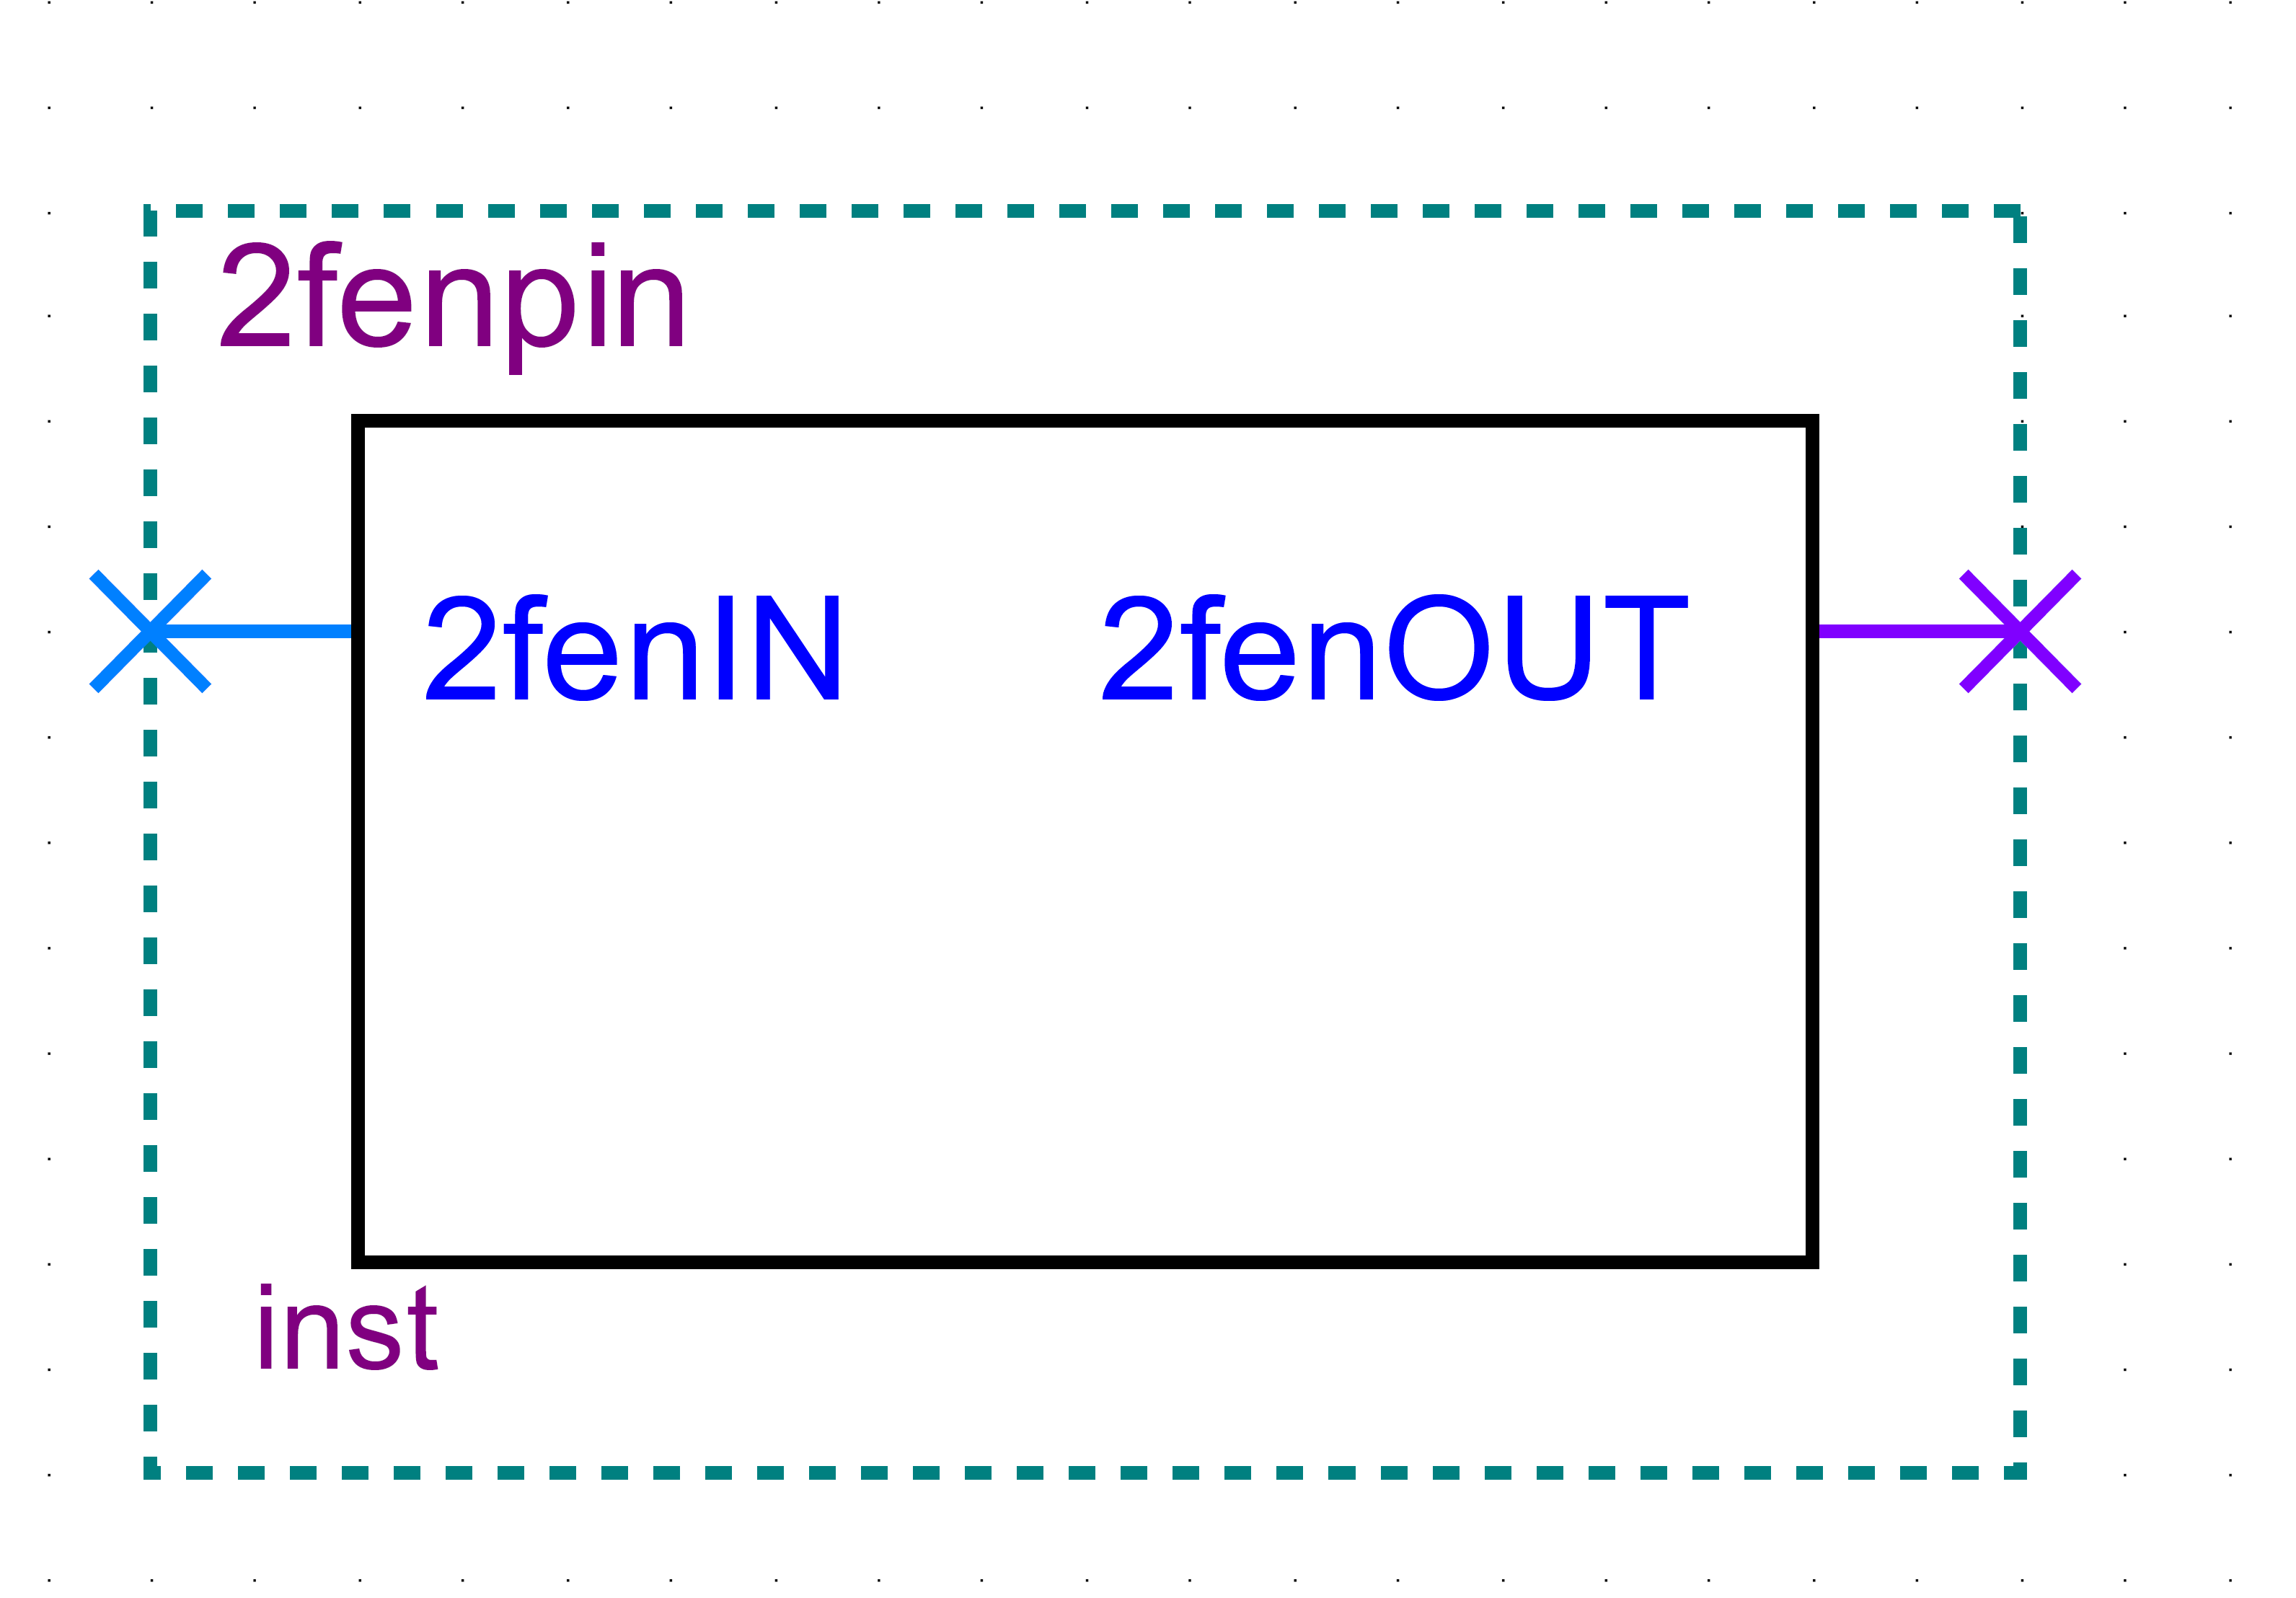
\includegraphics[width=0.3\textwidth]{picture/fenzhuang2fenp.png} 
	\caption{}
	\label{fig:fengzhuang2fenpin}   
\end{figure}
\subsubsection{4分频}
将2个二分频模块级联实现4分频,原理图见图\ref{fig:4fenpin},仿真波形见图\ref{fig:fangzhen4fenpin},封装图见图\ref{fig:fengzhuang4fenpin}。
\begin{figure}[hp]
	\centering  
	\includegraphics[width=0.8\textwidth]{picture/4fenpin.png} 
	\caption{}
	\label{fig:4fenpin}   
\end{figure}
\begin{figure}[hp]
	\centering  
	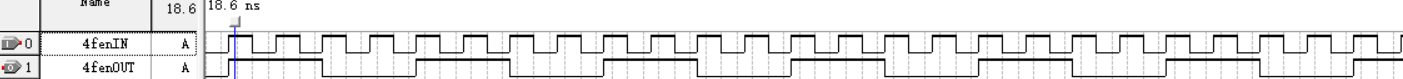
\includegraphics[width=\textwidth]{picture/TIM20181210161238.png} 
	\caption{}
	\label{fig:fangzhen4fenpin}   
\end{figure}
\begin{figure}[hp]
	\centering  
	\includegraphics[width=0.3\textwidth]{picture/fenzhuang4fenp.png} 
	\caption{}
	\label{fig:fengzhuang4fenpin}   
\end{figure}
\subsubsection{10分频}
借助74161芯片和2分频电路实现10分频,当74160计数到4时,同步置数到0,实现循环,同时输出1次高电平给2分频电路,实现占空比为$\frac{1}{2}$的10分频。原理图见图\ref{fig:10fenpin},仿真波形见图\ref{fig:fangzhen10fenpin},封装图见图\ref{fig:fengzhuang10fenpin}。
\begin{figure}[hp]
	\centering  
	\includegraphics[width=\textwidth]{picture/10fenpin.png} 
	\caption{}
	\label{fig:10fenpin}   
\end{figure}
\begin{figure}[hp]
	\centering  
	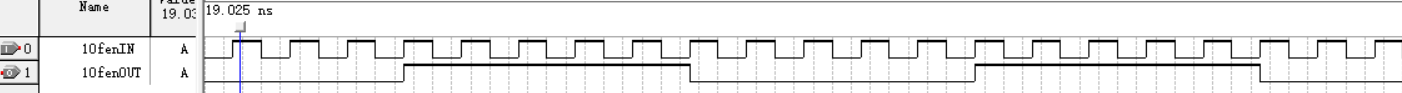
\includegraphics[width=\textwidth]{picture/TIM20181210165821.png} 
	\caption{}
	\label{fig:fangzhen10fenpin}   
\end{figure}
\begin{figure}[hp]
	\centering  
	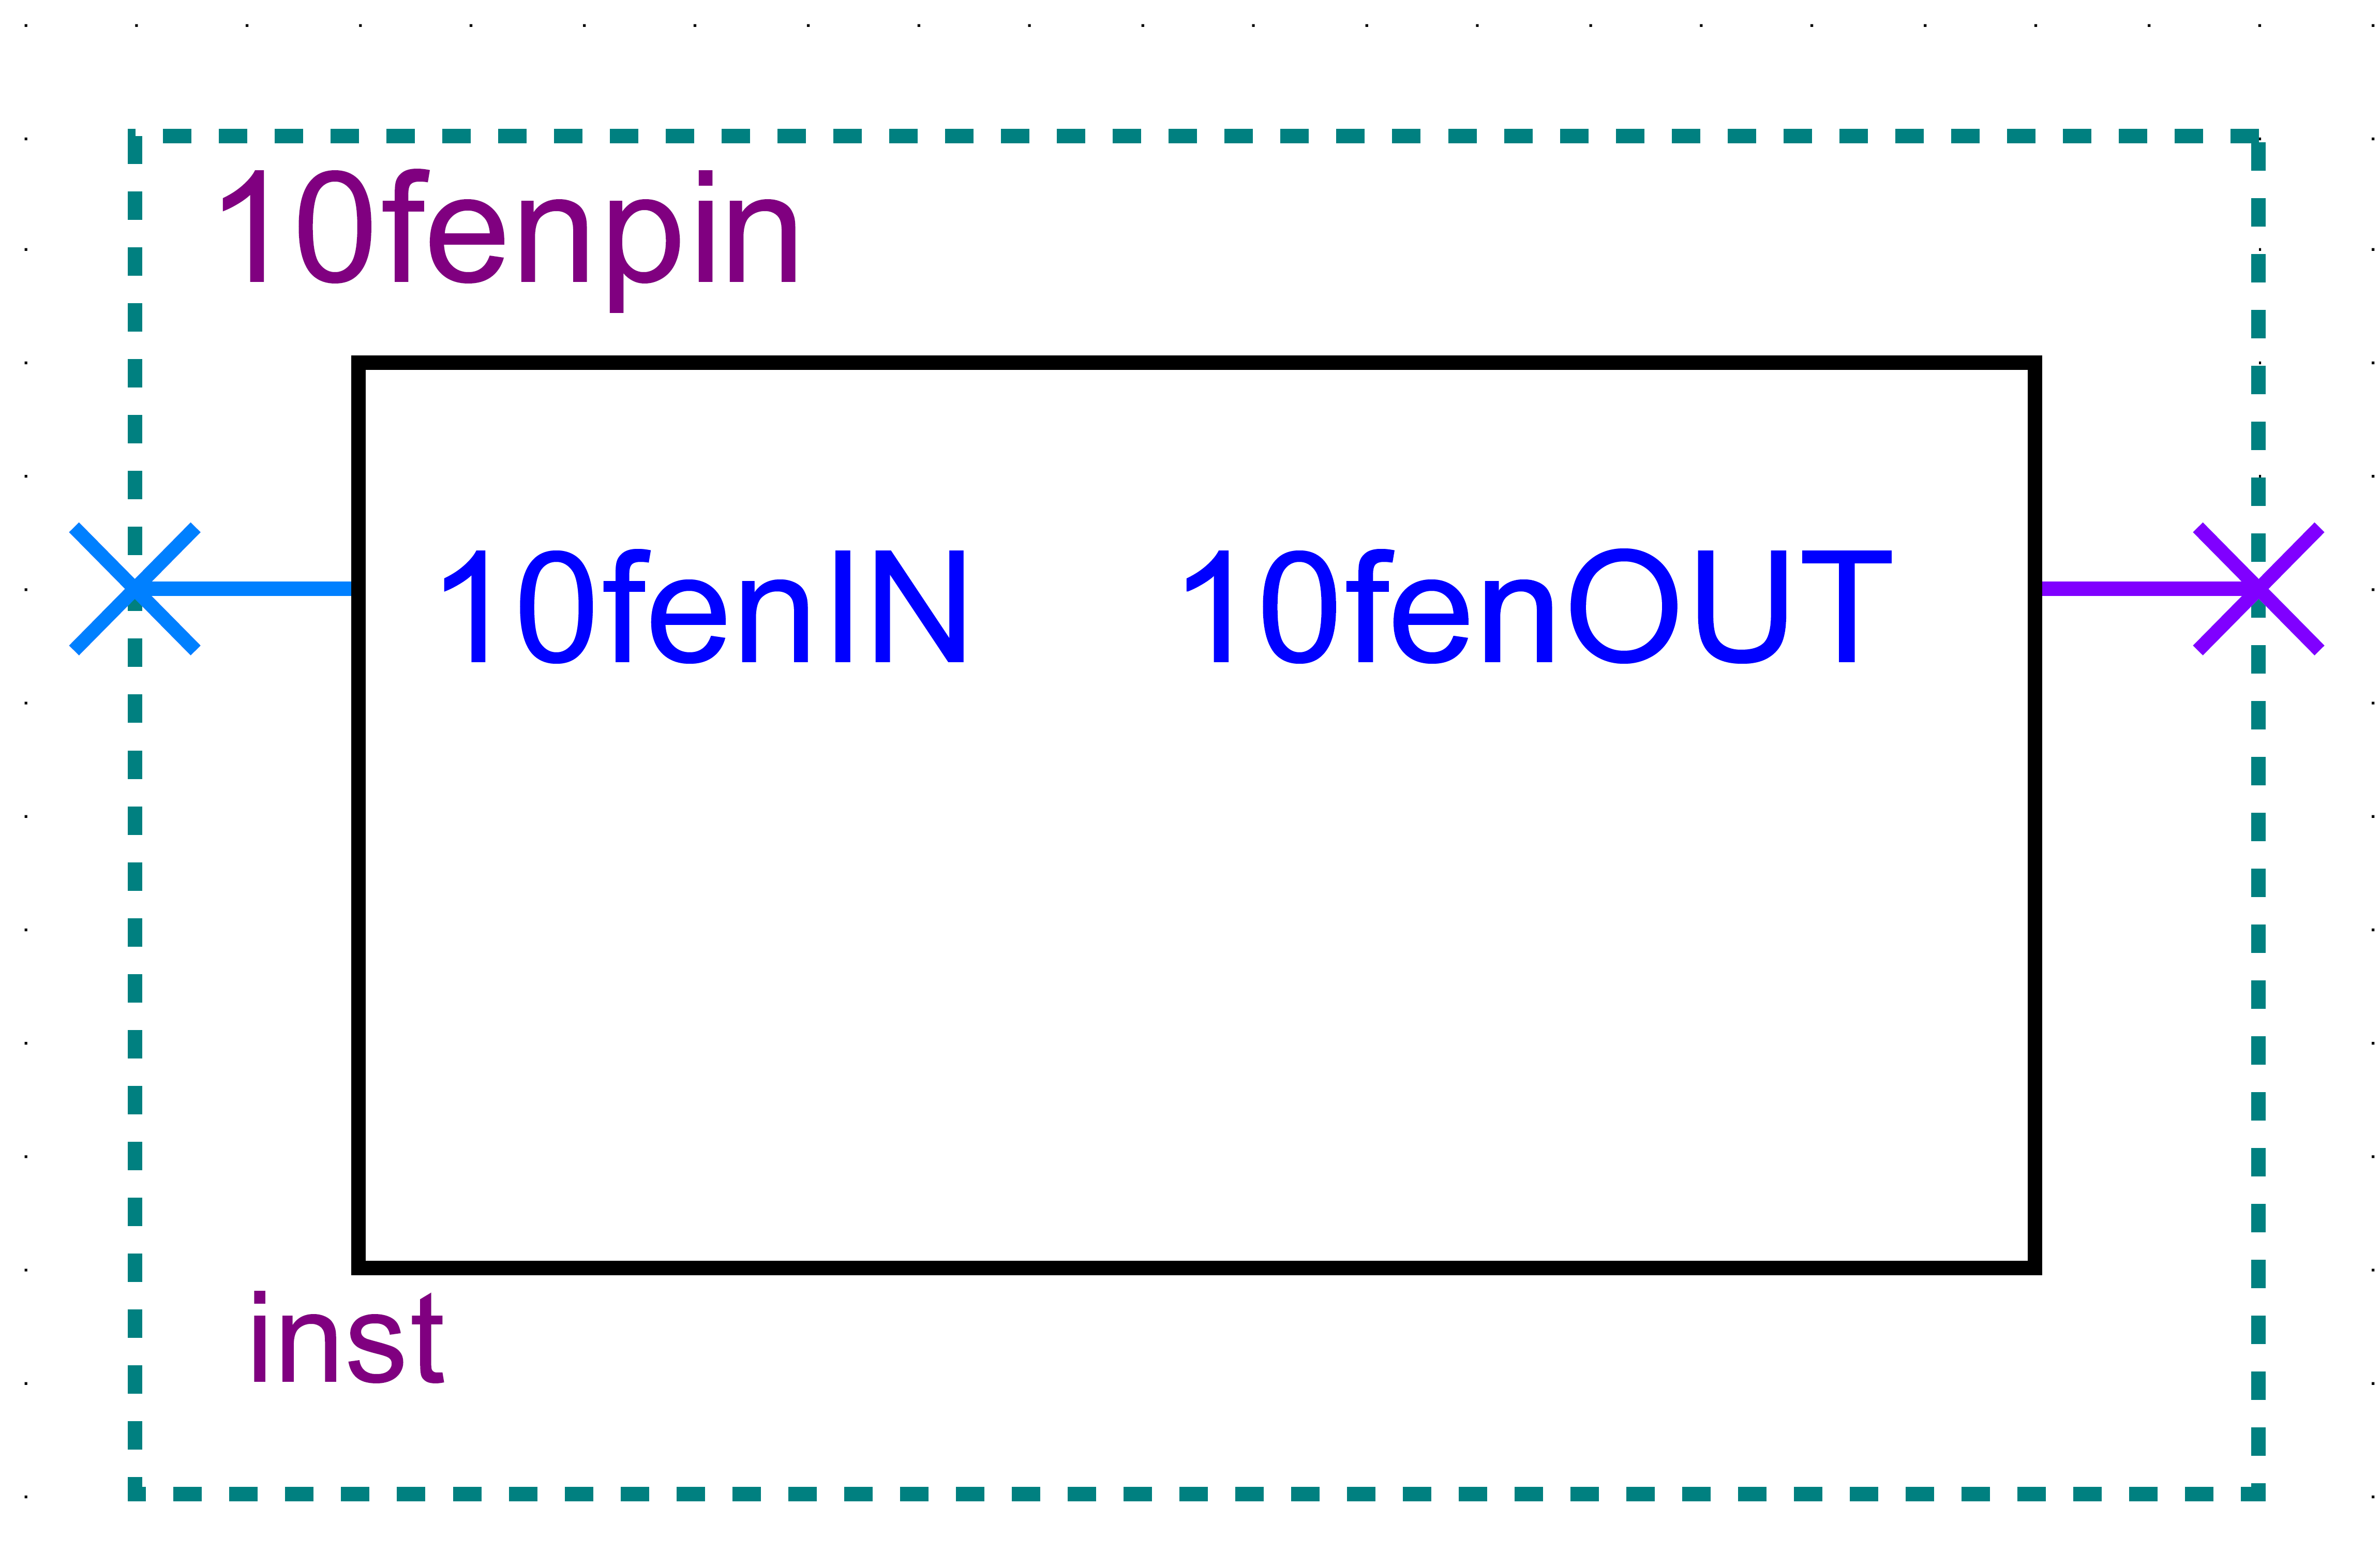
\includegraphics[width=0.3\textwidth]{picture/fenzhuang10fenp.png} 
	\caption{}
	\label{fig:fengzhuang10fenpin}   
\end{figure}
\subsubsection{12分频}
借助74161芯片实现12分频,当74161计数到11时,同步置数到0,实现循环,同时输出1次高电平,实现分频。原理图见图\ref{fig:12fenpin},仿真波形见图\ref{fig:fangzhen12fenpin},封装图见图\ref{fig:fengzhuang12fenpin}。
\begin{figure}[hp]
	\centering  
	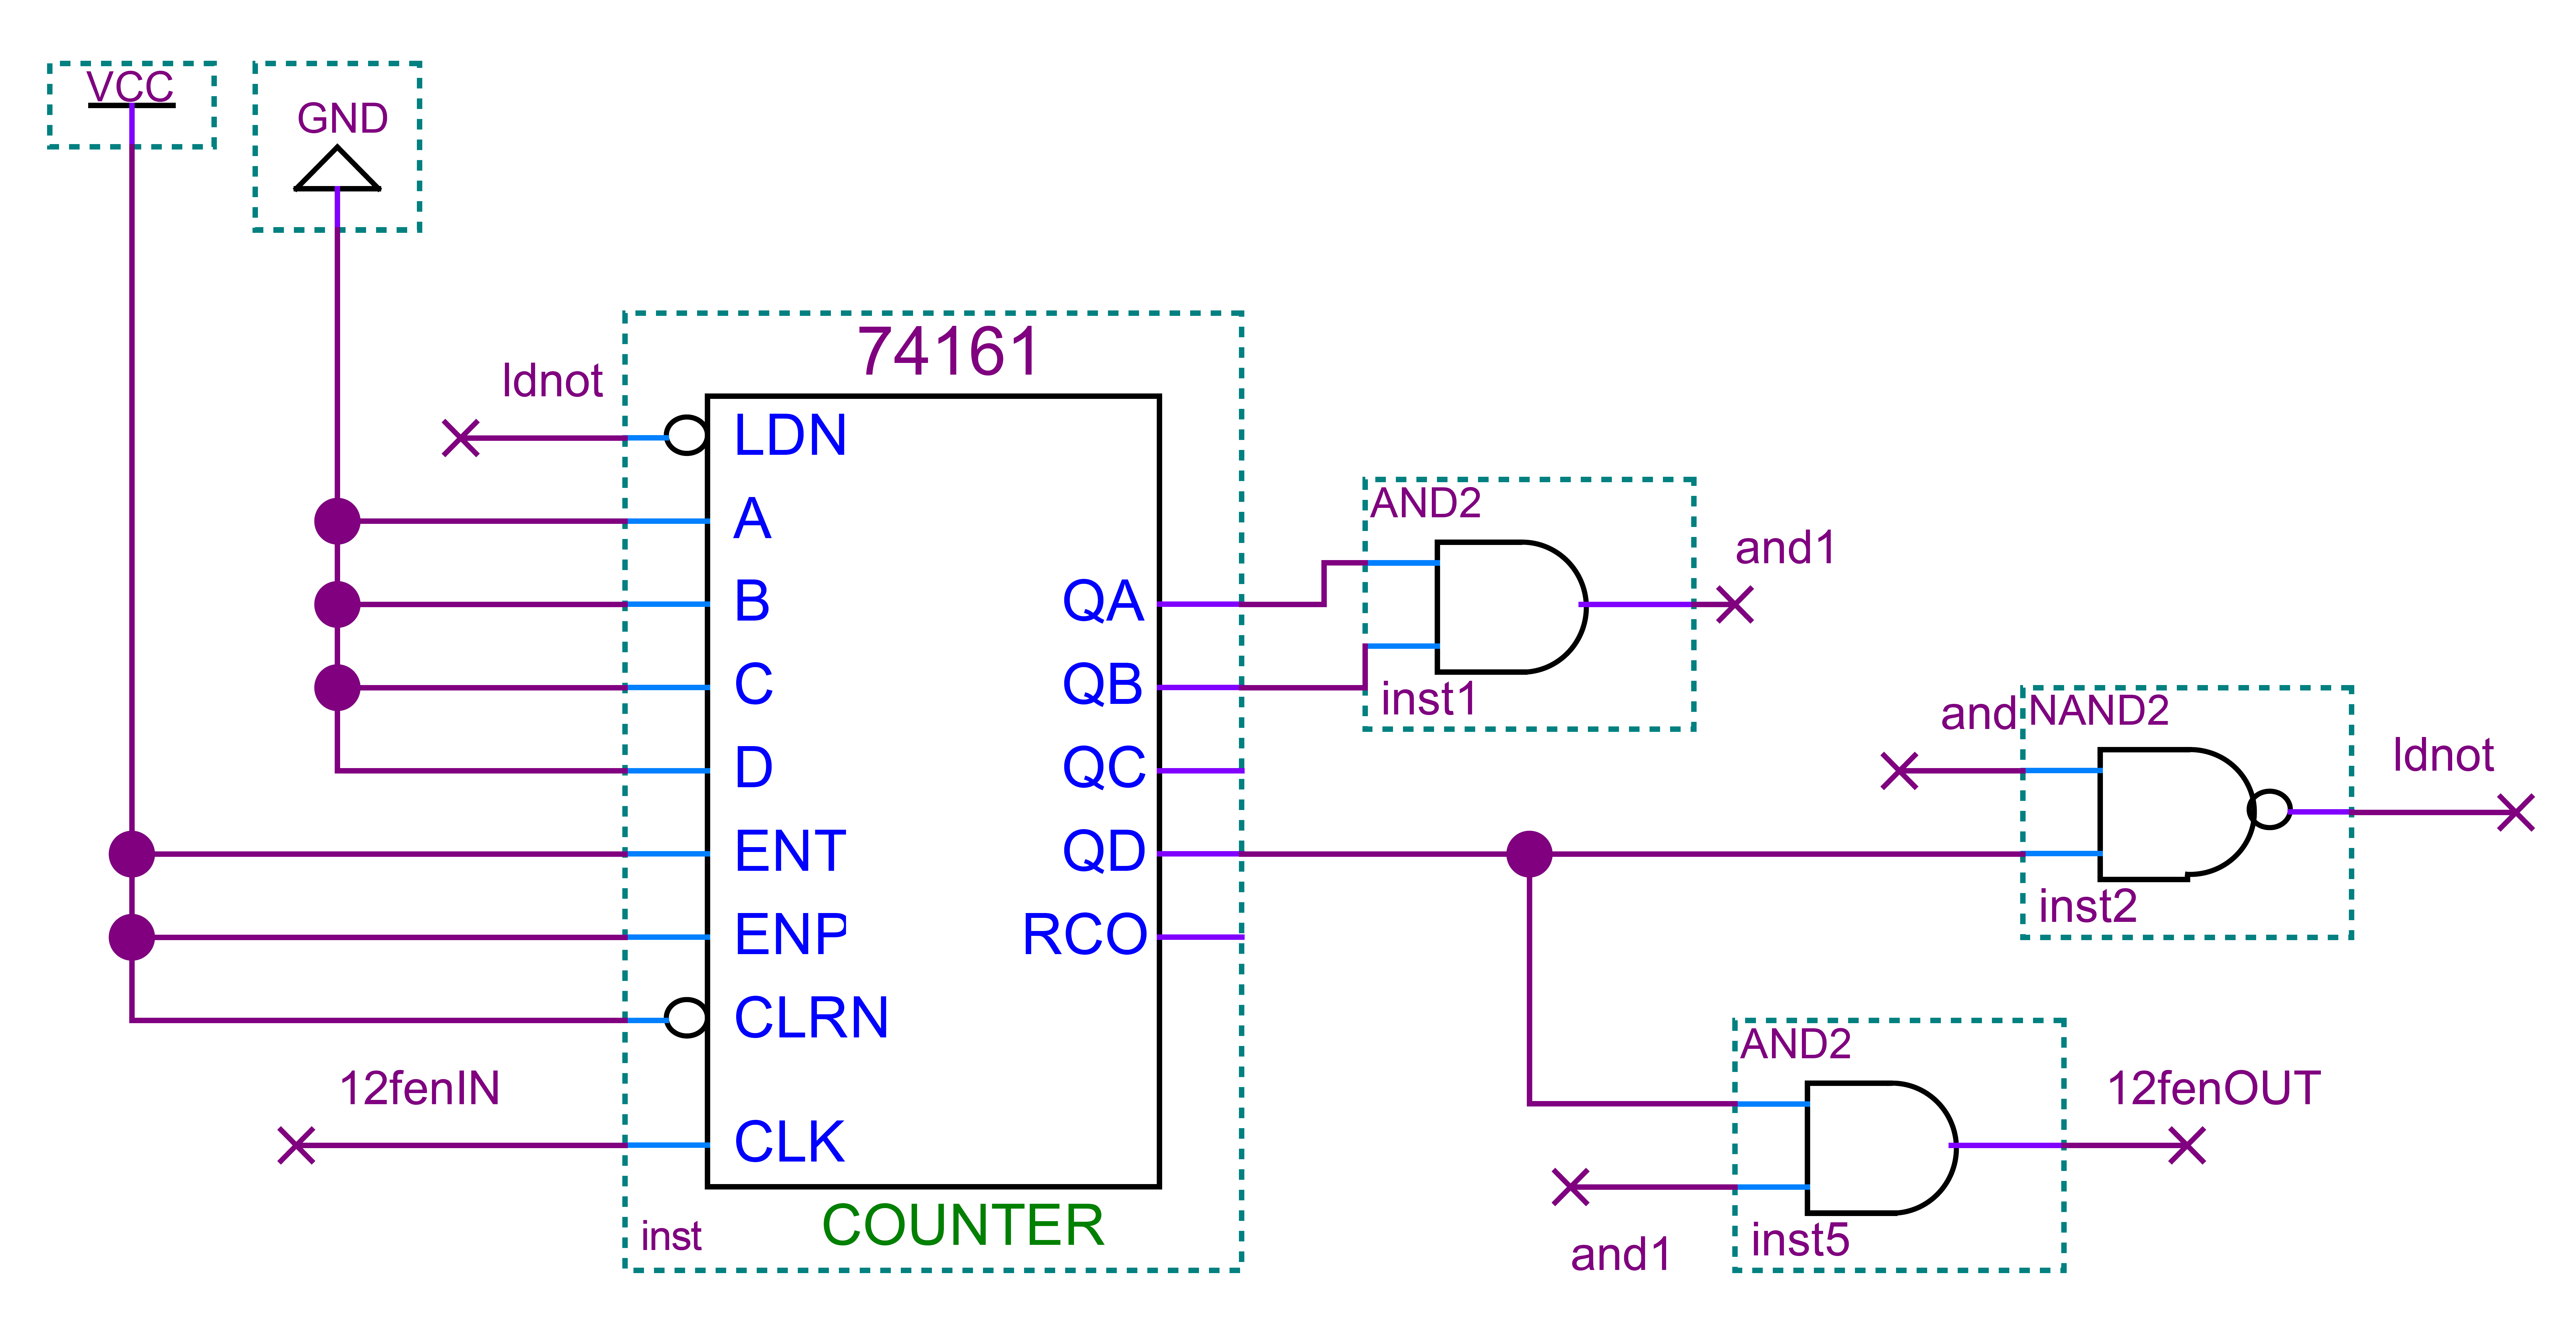
\includegraphics[width=\textwidth]{picture/12fenp.png} 
	\caption{}
	\label{fig:12fenpin}   
\end{figure}
\begin{figure}[hp]
	\centering  
	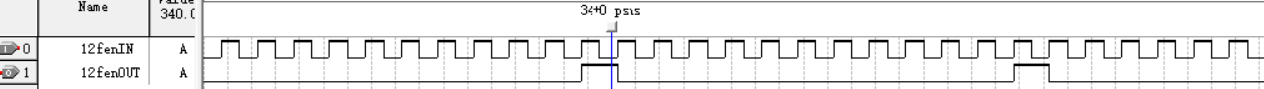
\includegraphics[width=\textwidth]{picture/TIM20181210160106.png} 
	\caption{}
	\label{fig:fangzhen12fenpin}   
\end{figure}
\begin{figure}[hp]
	\centering  
	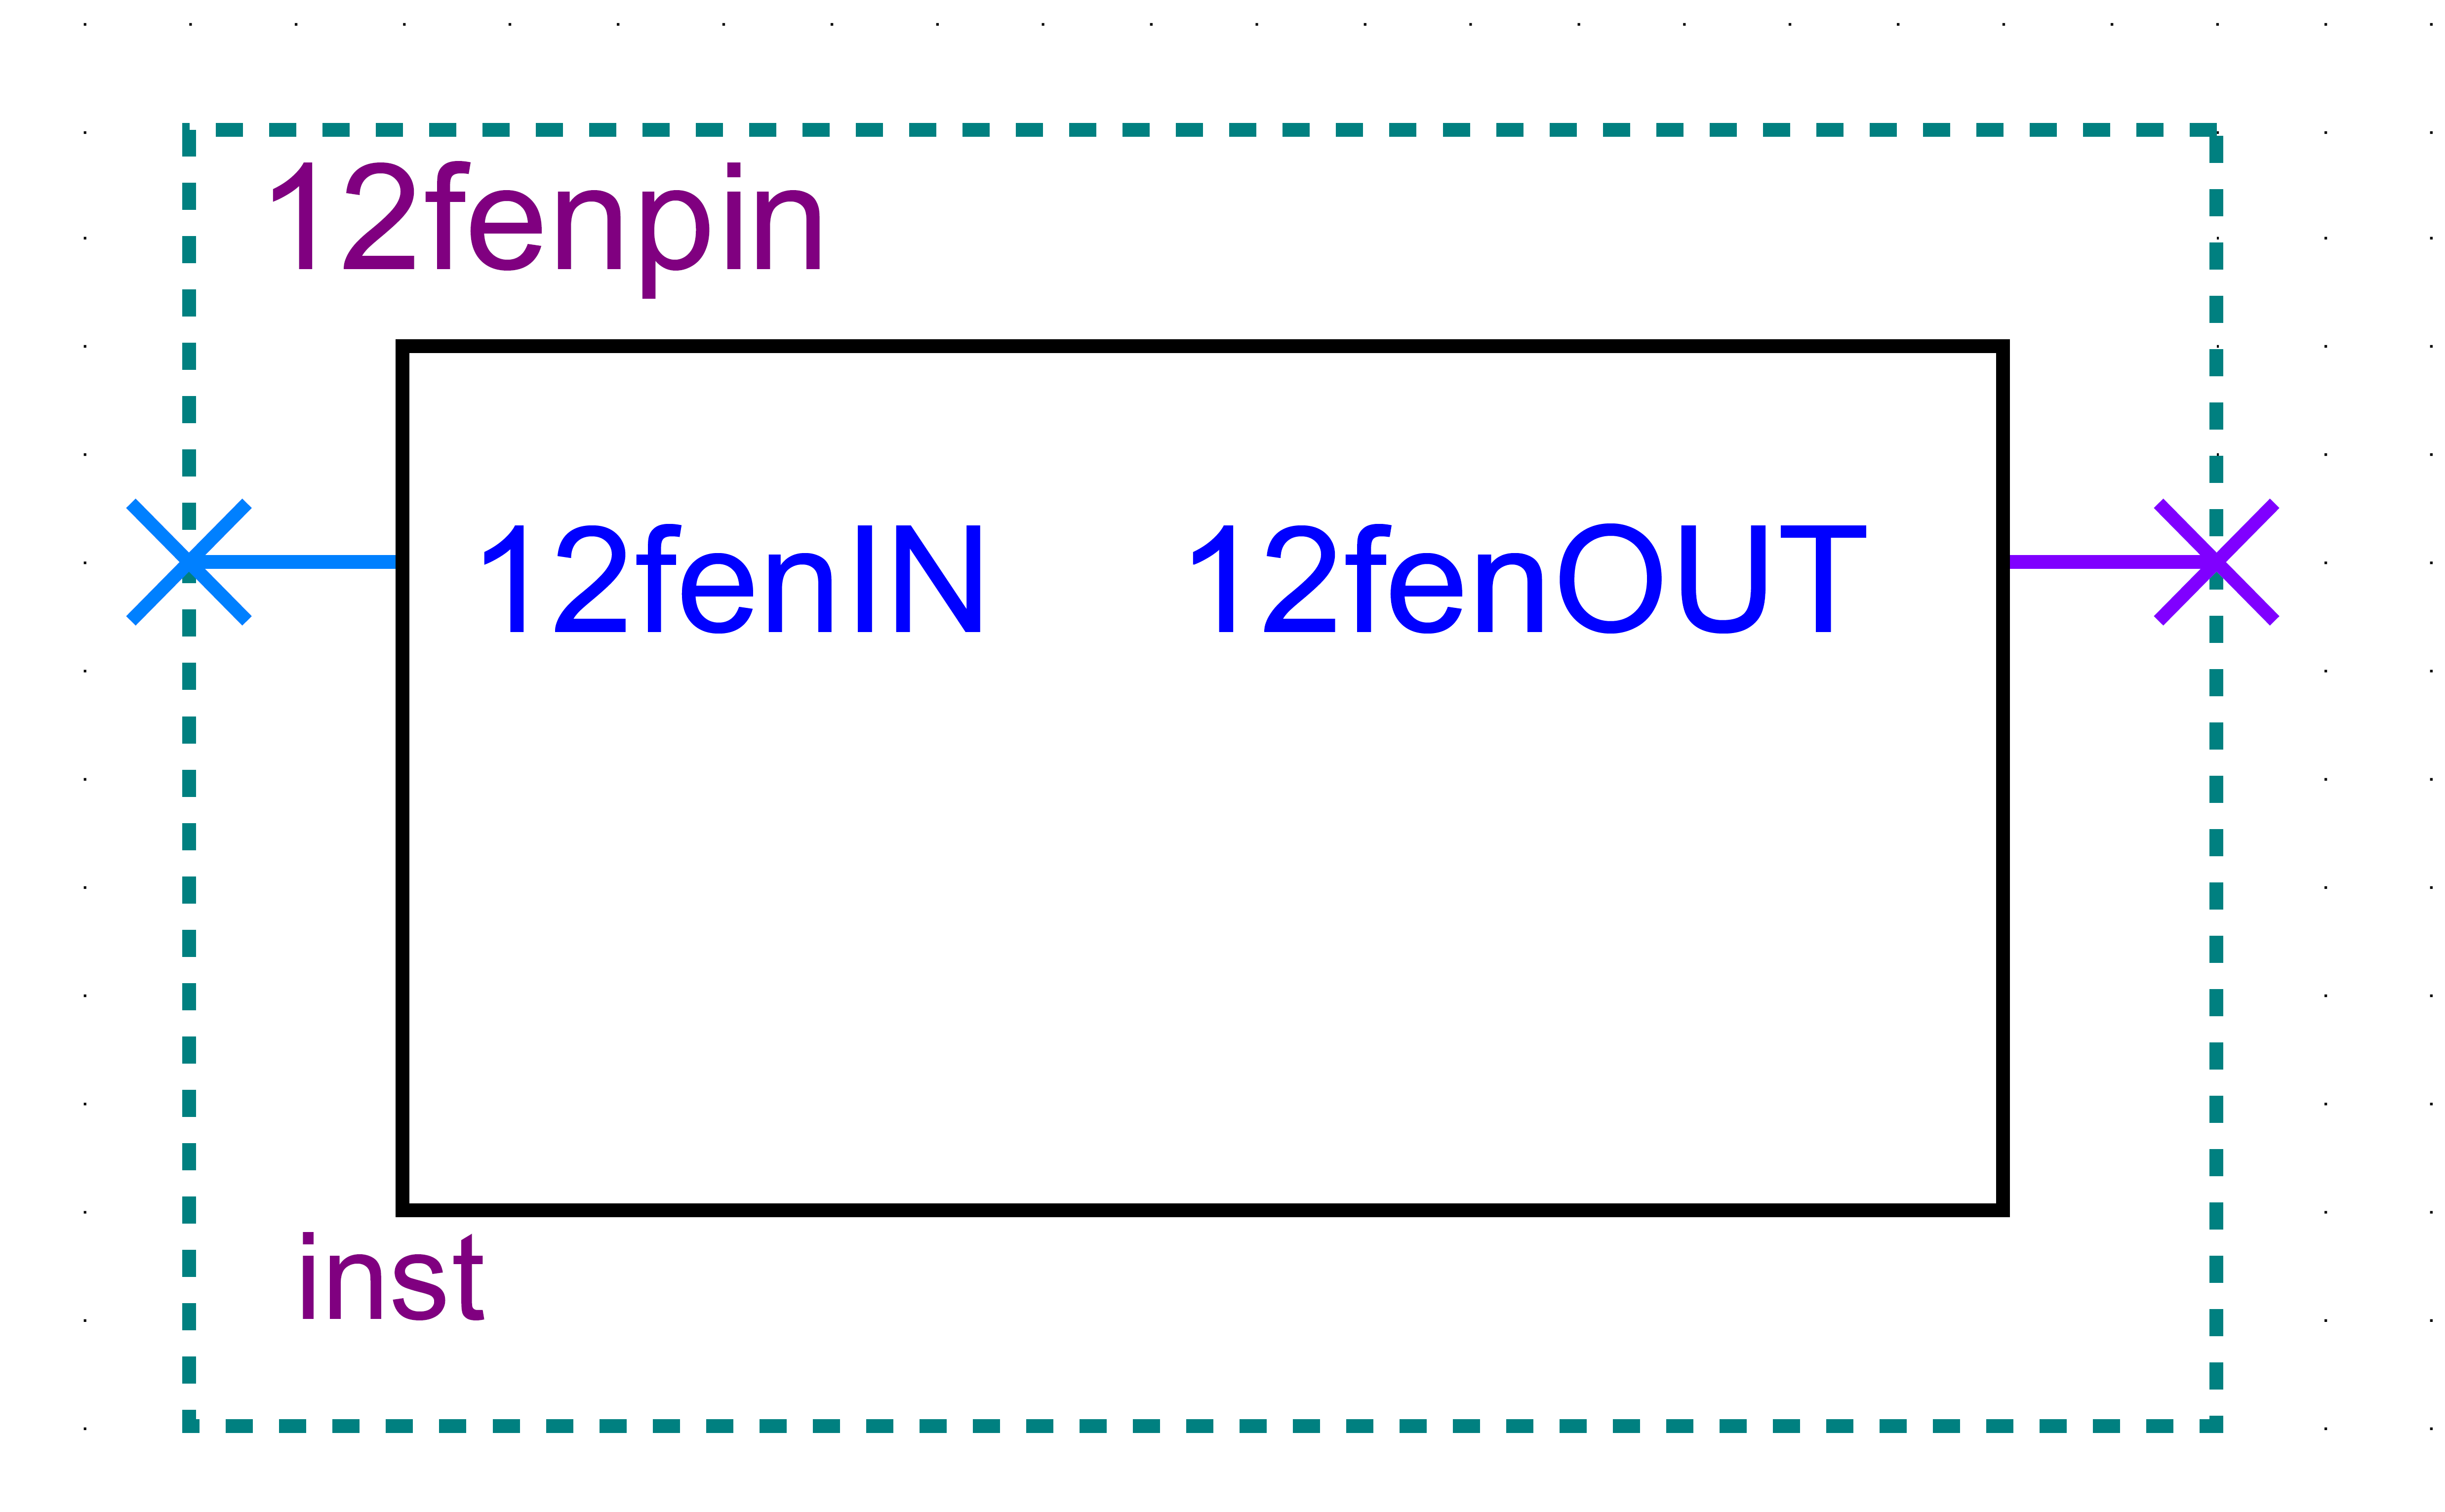
\includegraphics[width=0.3\textwidth]{picture/fenzhuang12fenp.png} 
	\caption{}
	\label{fig:fengzhuang12fenpin}   
\end{figure}
\subsubsection{1000分频}
将3个10分频级联,得到1000分频。原理图见图\ref{fig:1000fenpin},封装图见图\ref{fig:fengzhuang1000fenpin}。
\begin{figure}[hp]
	\centering  
	\includegraphics[width=\textwidth]{picture/1000fenpin.png} 
	\caption{}
	\label{fig:1000fenpin}   
\end{figure}
\begin{figure}[hp]
	\centering  
	\includegraphics[width=0.3\textwidth]{picture/fenzhuang1000fenp.png} 
	\caption{}
	\label{fig:fengzhuang1000fenpin}   
\end{figure}
\subsubsection{分频模块}
最终,通过级联以上的各种分频器,实现分频模块。原理图见图\ref{fig:allfenpin},仿真波形大致情况见图\ref{fig:fangzhenallfenpin},封装图见图\ref{fig:fengzhuangallfenpin}。
\begin{figure}[hp]
	\centering  
	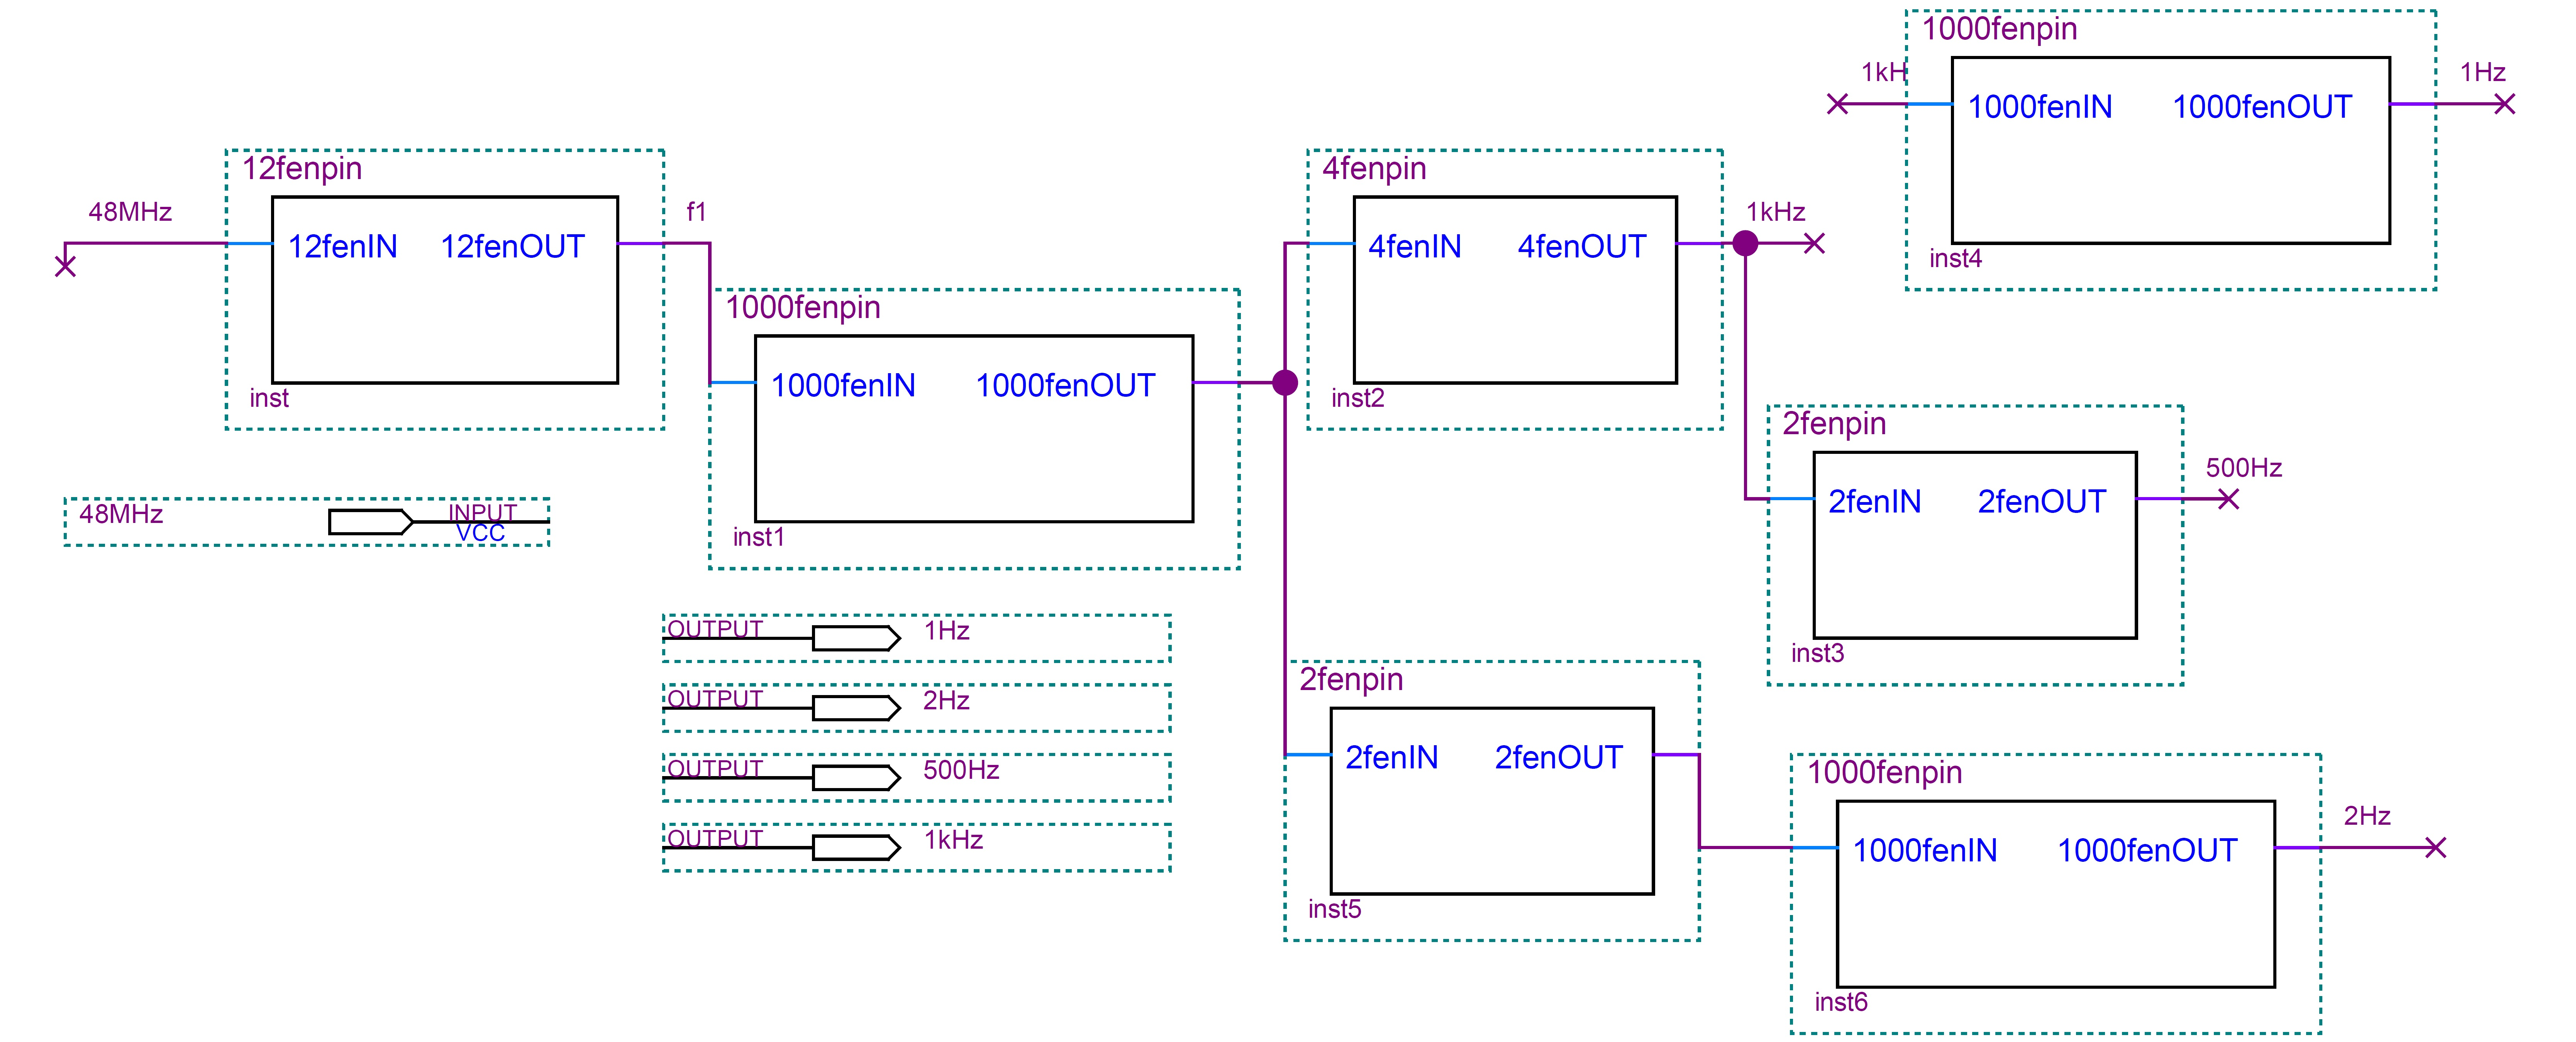
\includegraphics[width=\textwidth]{picture/fenpin.jpg} 
	\caption{}
	\label{fig:allfenpin}   
\end{figure}
\begin{figure}[hp]
	\centering  
	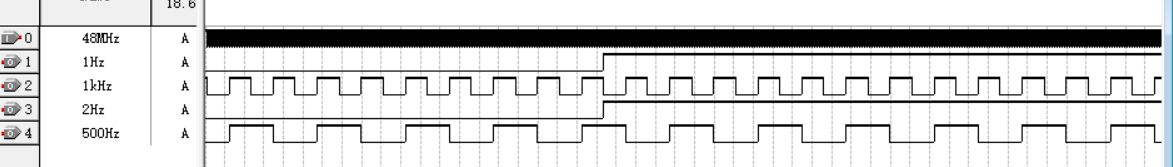
\includegraphics[width=\textwidth]{picture/TIM20181210184848.png} 
	\caption{}
	\label{fig:fangzhenallfenpin}   
\end{figure}
\begin{figure}[hp]
	\centering  
	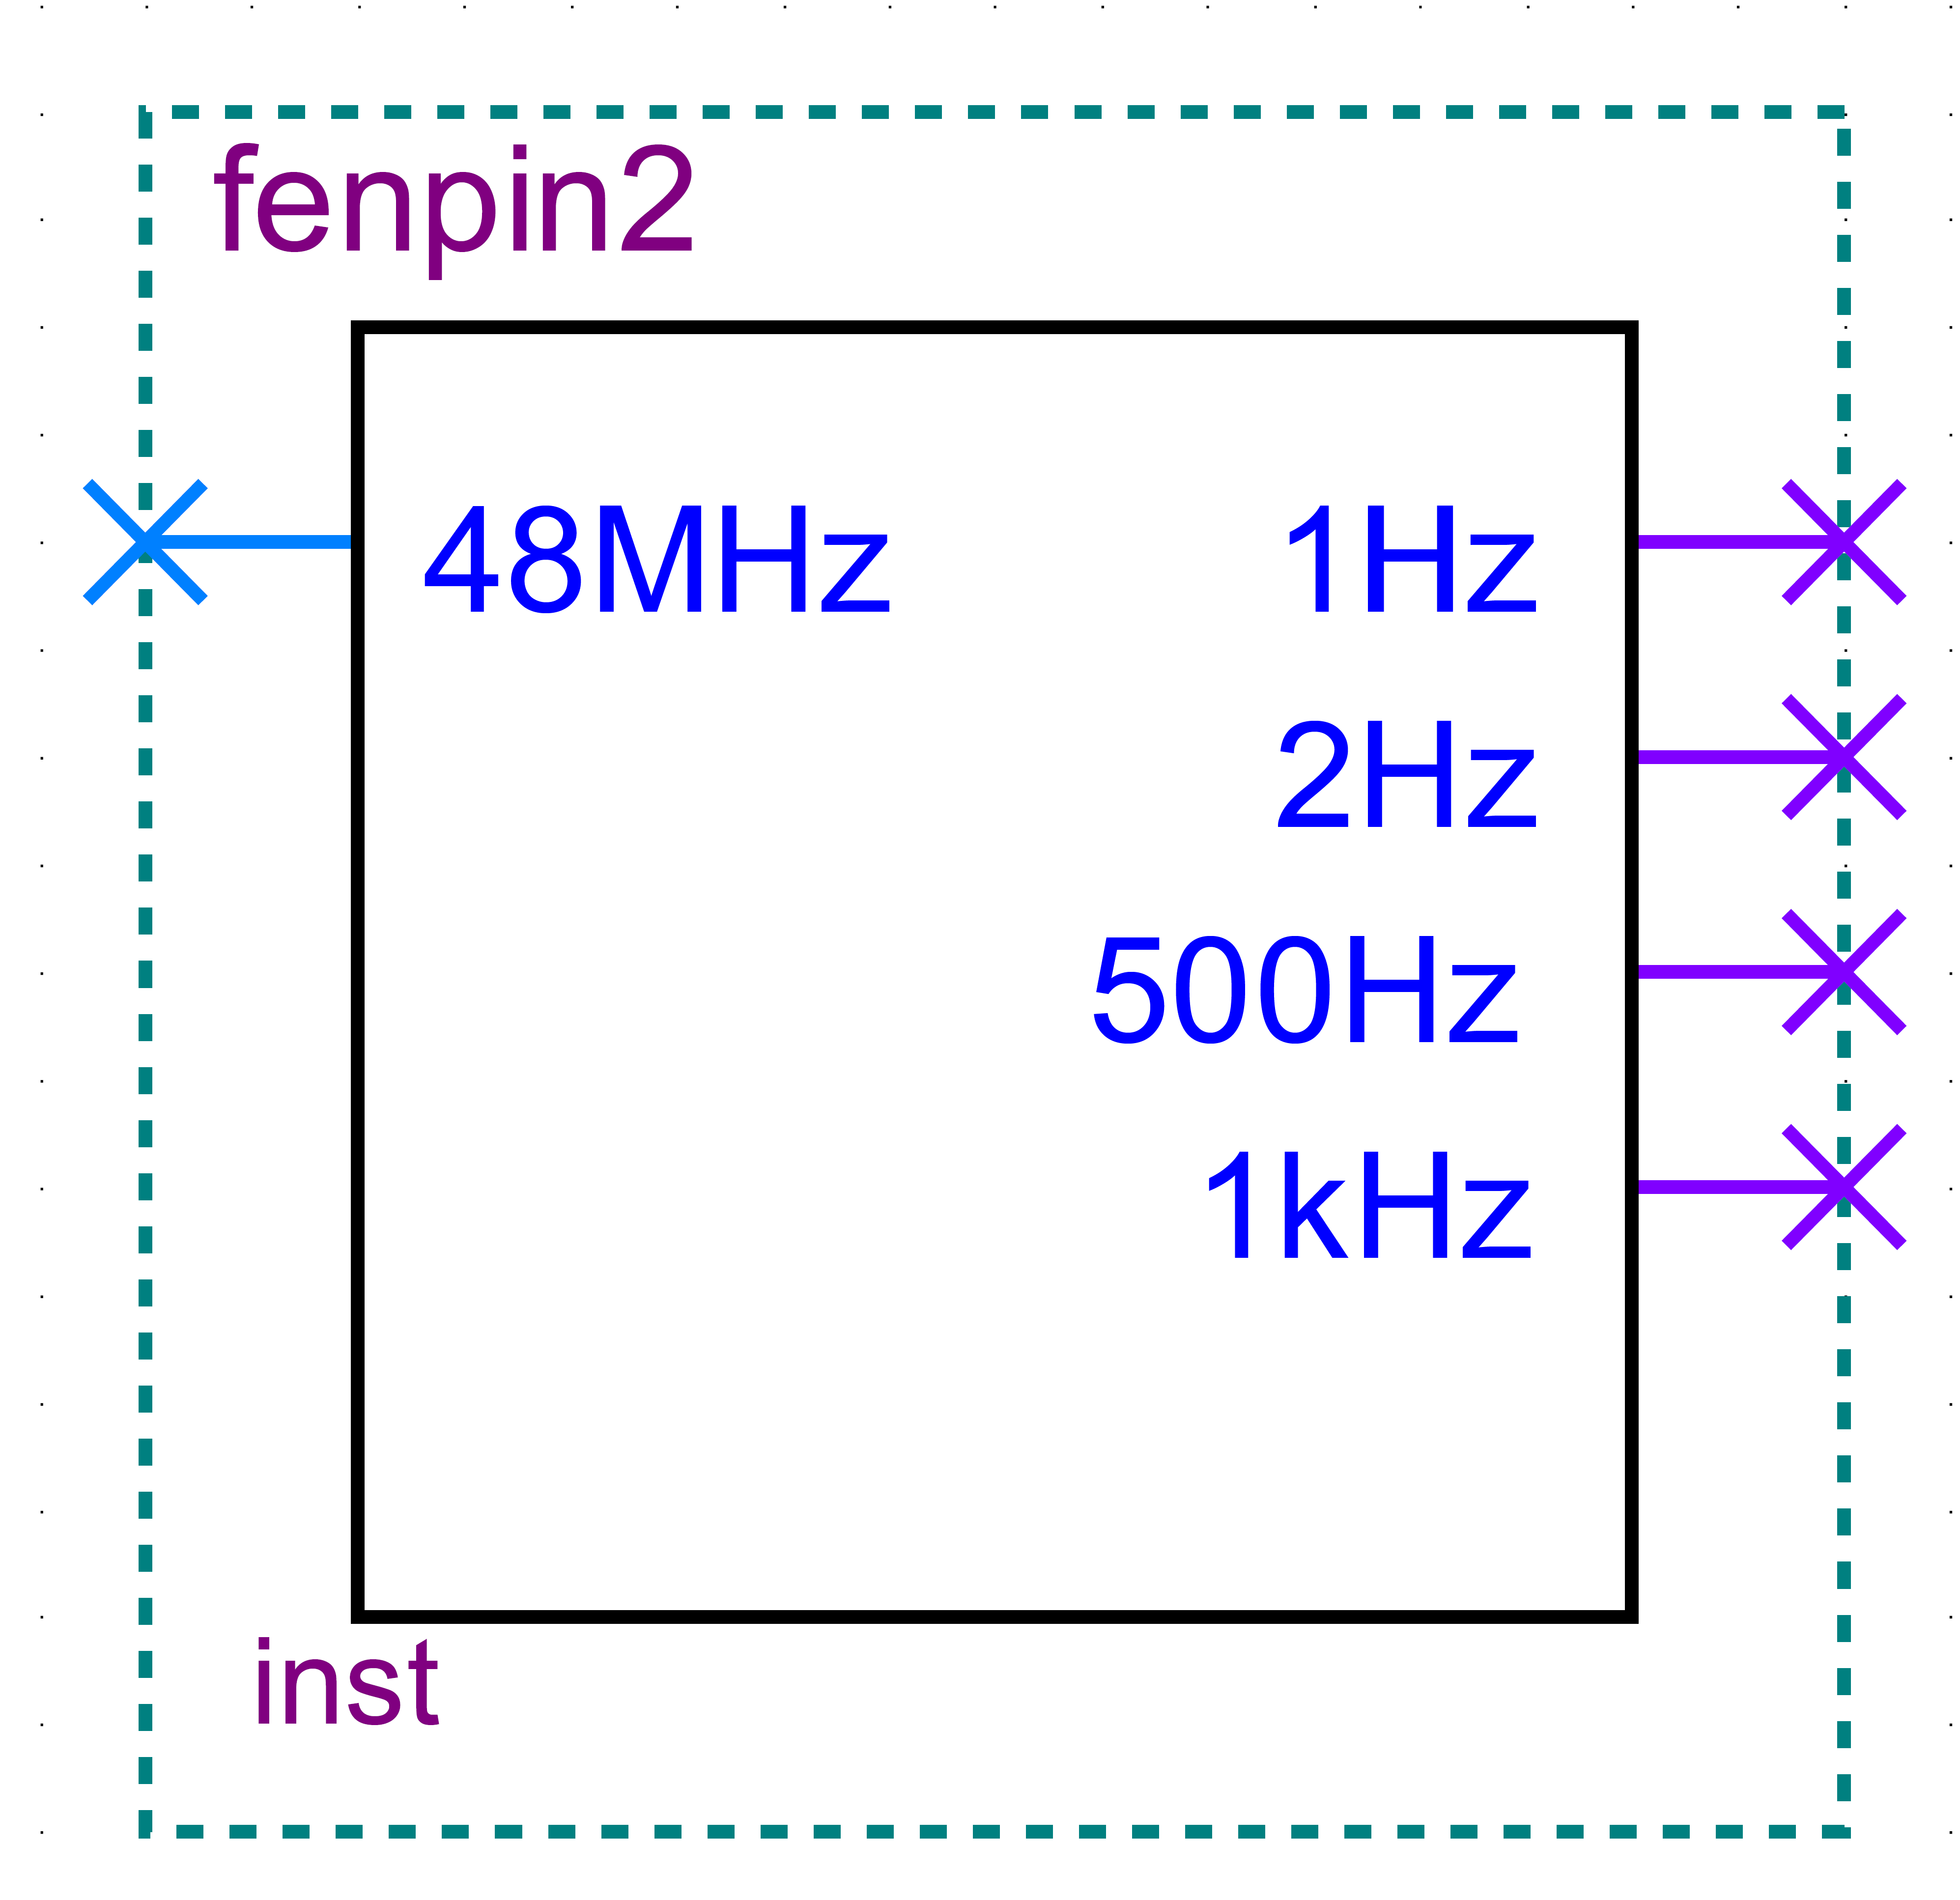
\includegraphics[width=0.3\textwidth]{picture/fenzhuangallfenp.png} 
	\caption{}
	\label{fig:fengzhuangallfenpin}   
\end{figure}

\subsection{总计时模块}
\subsubsection{由模7、模24、模60模块组成的基本计时模块}
利用VHDL语言的IF语句,对计数的条件进行判断。例如模7,则在计数到0111(7)时跳转到0001,即可实现数字1到7的循环计数。mo24,mo60的代码也类似,只是判断的条件不同。\par
\paragraph{VHDL代码实现模7}模7的代码如下,仿真情况见图\ref{fig:fangzhenmo7},封装图见图\ref{fig:fengzhuangmo7}。
\begin{lstlisting}[language=VHDL]
library ieee;
use ieee.std_logic_1164.all;
use ieee.std_logic_unsigned.all;
ENTITY mo7 IS 
 PORT
( en   :IN  std_logic;
clear:IN  std_logic;--when 0,output is always 0
clk  :IN  std_logic;
ql :buffer std_logic_vector(3 downto 0)
);
END mo7;
ARCHITECTURE beh OF mo7 IS
BEGIN
PROCESS(clk,clear)
BEGIN
IF(clear='0')THEN
ql<="0000";
ELSIF(clk'EVENT AND clk='1')THEN
if(en='1')then
if(ql=7) then
ql<="0001";
else
ql<=ql+1;
end if;
end if;
END IF;
END PROCESS;
END beh;
} 
\end{lstlisting} 
\begin{figure}[hp]
	\centering  
	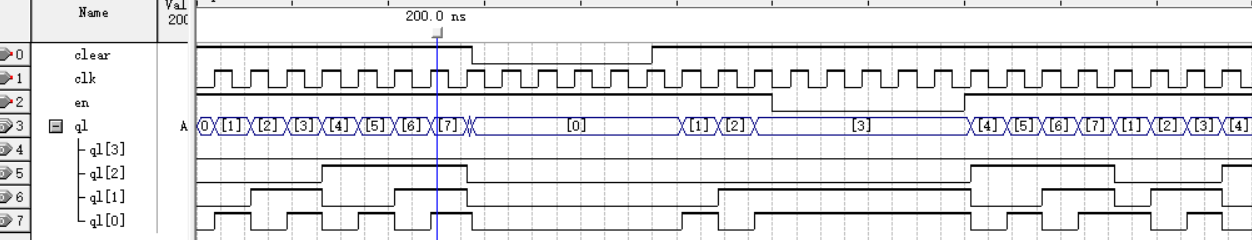
\includegraphics[width=\textwidth]{picture/TIM20181210201132.png} 
	\caption{}
	\label{fig:fangzhenmo7}   
\end{figure}
\begin{figure}[hp]
	\centering  
	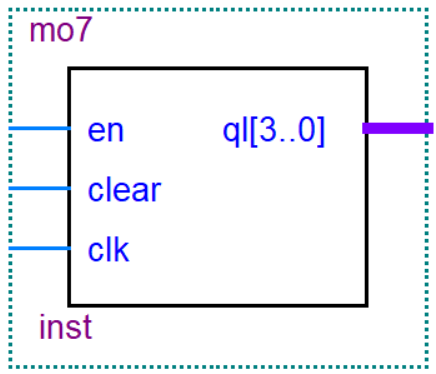
\includegraphics[width=0.3\textwidth]{picture/fenzhuangmo7.png} 
	\caption{}
	\label{fig:fengzhuangmo7}   
\end{figure}\par
\paragraph{VHDL代码实现模24}模24的代码如下,仿真情况见图\ref{fig:fangzhenmo24},封装图见图\ref{fig:fengzhuangmo24}。
\begin{lstlisting}[language=VHDL]
library ieee;
use ieee.std_logic_1164.all;
use ieee.std_logic_unsigned.all;
ENTITY mo24 IS 
 PORT
( en   :IN  std_logic;
clear:IN  std_logic;--when 0,output is always 0
clk  :IN  std_logic;
cout :out  std_logic;--jinwei output
qh :buffer std_logic_vector(3 downto 0);--shiwei output
ql :buffer std_logic_vector(3 downto 0)
);--gewei output
END mo24;
ARCHITECTURE beh OF mo24 IS
BEGIN
cout<='1'when(qh="0010"and ql="0011"and en='1')else'0'; 

PROCESS(clk,clear)
BEGIN
IF(clear='0')THEN
qh<="0000";
ql<="0000";
ELSIF(clk'EVENT AND clk='1')THEN
if(en='1')then
if((ql=3 and qh=2) or ql=9) then
ql<="0000";
if(qh=2)then
qh<="0000";
else
qh<=qh+1;
end if;
else
ql<=ql+1;
end if;
end if;
END IF;
END PROCESS;
END beh;
\end{lstlisting} 
\begin{figure}[hp]
	\centering  
	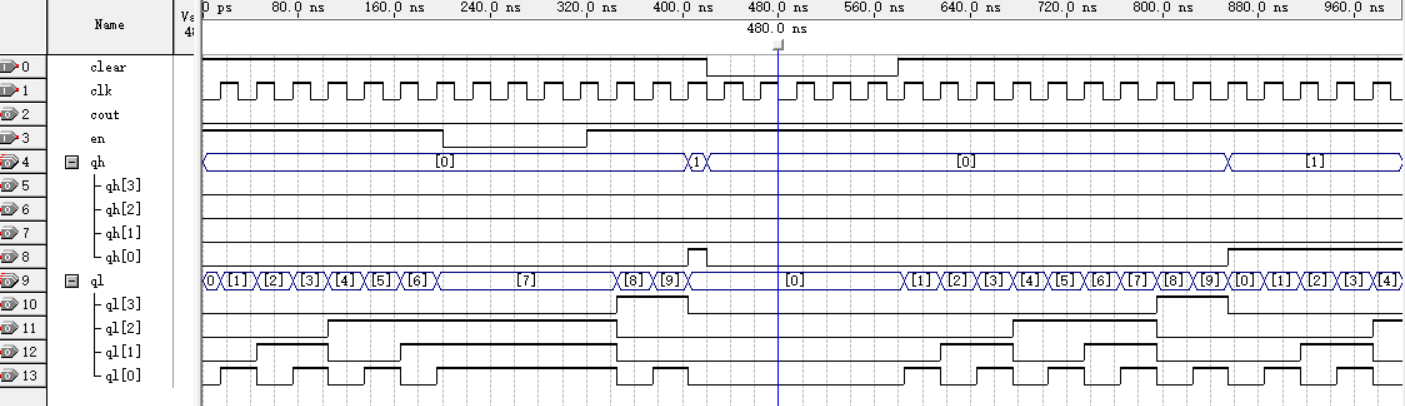
\includegraphics[width=\textwidth]{picture/TIM20181210203225.png} 
	\caption{}
	\label{fig:fangzhenmo24}   
\end{figure}
\begin{figure}[hp]
	\centering  
	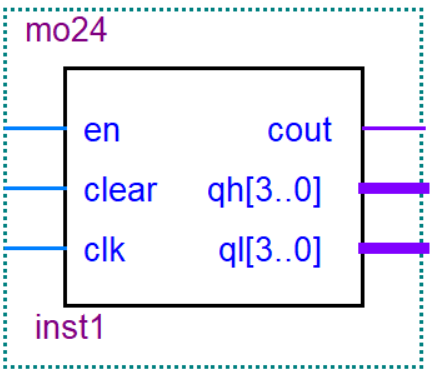
\includegraphics[width=0.3\textwidth]{picture/fenzhuangmo24.png} 
	\caption{}
	\label{fig:fengzhuangmo24}   
\end{figure}\par
\paragraph{VHDL代码实现模60}模60的代码如下,仿真情况见图\ref{fig:fangzhenmo60},封装图见图\ref{fig:fengzhuangmo60}。
\begin{lstlisting}[language=VHDL]
library ieee;
use ieee.std_logic_1164.all;
use ieee.std_logic_unsigned.all;
ENTITY mo60 IS 
 PORT
( en   :IN  std_logic;
clear:IN  std_logic;--when 0,output is always 0
clk  :IN  std_logic;
cout :out  std_logic;--jinwei output
qh :buffer std_logic_vector(3 downto 0);--shiwei output
ql :buffer std_logic_vector(3 downto 0)
);--gewei output
END mo60;
ARCHITECTURE beh OF mo60 IS
BEGIN
cout<='1'when(qh="0101"and ql="1001"and en='1')else'0'; 

PROCESS(clk,clear)
BEGIN
IF(clear='0')THEN
qh<="0000";
ql<="0000";
ELSIF(clk'EVENT AND clk='1')THEN
if(en='1')then
if(ql=9) then
ql<="0000";
if(qh=5 and ql=9 )then
qh<="0000";
else
qh<=qh+1;
end if;
else
ql<=ql+1;
end if;
end if;
END IF;
END PROCESS;
END beh;
\end{lstlisting} 
\begin{figure}[hp]
	\centering  
	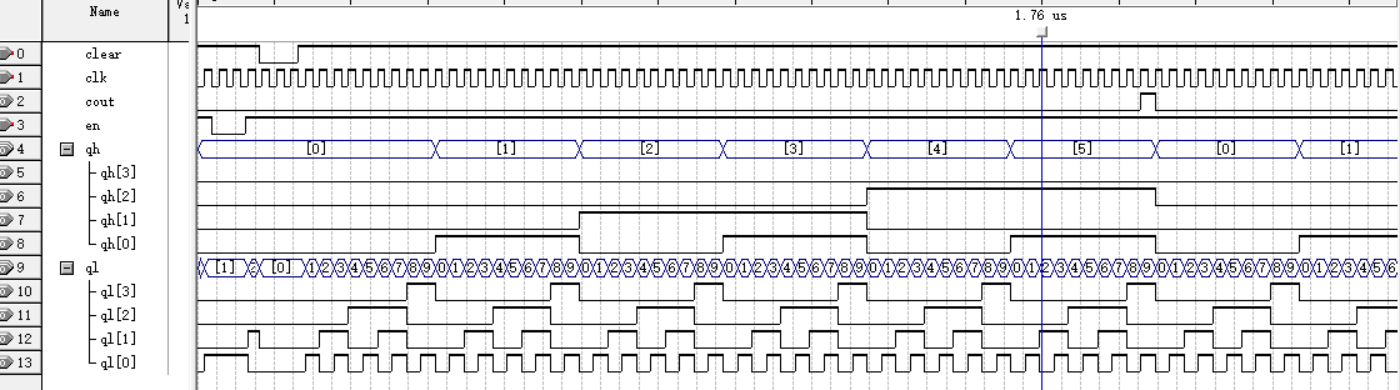
\includegraphics[width=\textwidth]{picture/TIM20181210205015.png} 
	\caption{}
	\label{fig:fangzhenmo60}   
\end{figure}
\begin{figure}[hp]
	\centering  
	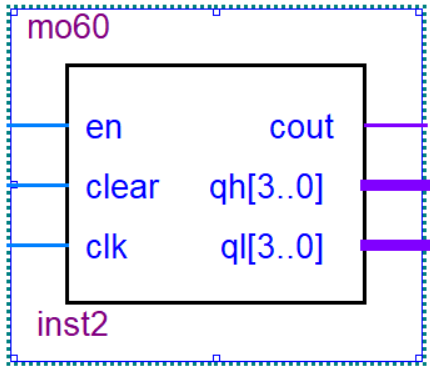
\includegraphics[width=0.3\textwidth]{picture/fenzhuangmo60.png} 
	\caption{}
	\label{fig:fengzhuangmo60}   
\end{figure}\par
\subsubsection{校时模块}
校时由二输入与门、非门和或门这三种逻辑门构成。当$K_3=0$(分位校时开关)时,时钟端clk输入1Hz的信号,时钟正常计数,当$K_3=1$时,时钟端clk输入2Hz的信号,进行快速校分。原理图见图\ref{fig:jiao},仿真情况见图\ref{fig:fzjiao},封装图见图\ref{fig:fengzhuangjiao}。\par对星期位、时位的校时电路原理类似,这里不赘述。\par 而事实上,为了实现同步时序基本计时,在基本计时模块,是将低位的进位信号作为高位的使能信号来实现时钟信号同步的,仅仅是改变时钟端信号并不能实现校时,还需要使能端的配合。由于对使能端的操作也涉及到保持功能,因此我将使能端的处理放在清零、保持模块完成。
\begin{figure}[hp]
	\centering  
	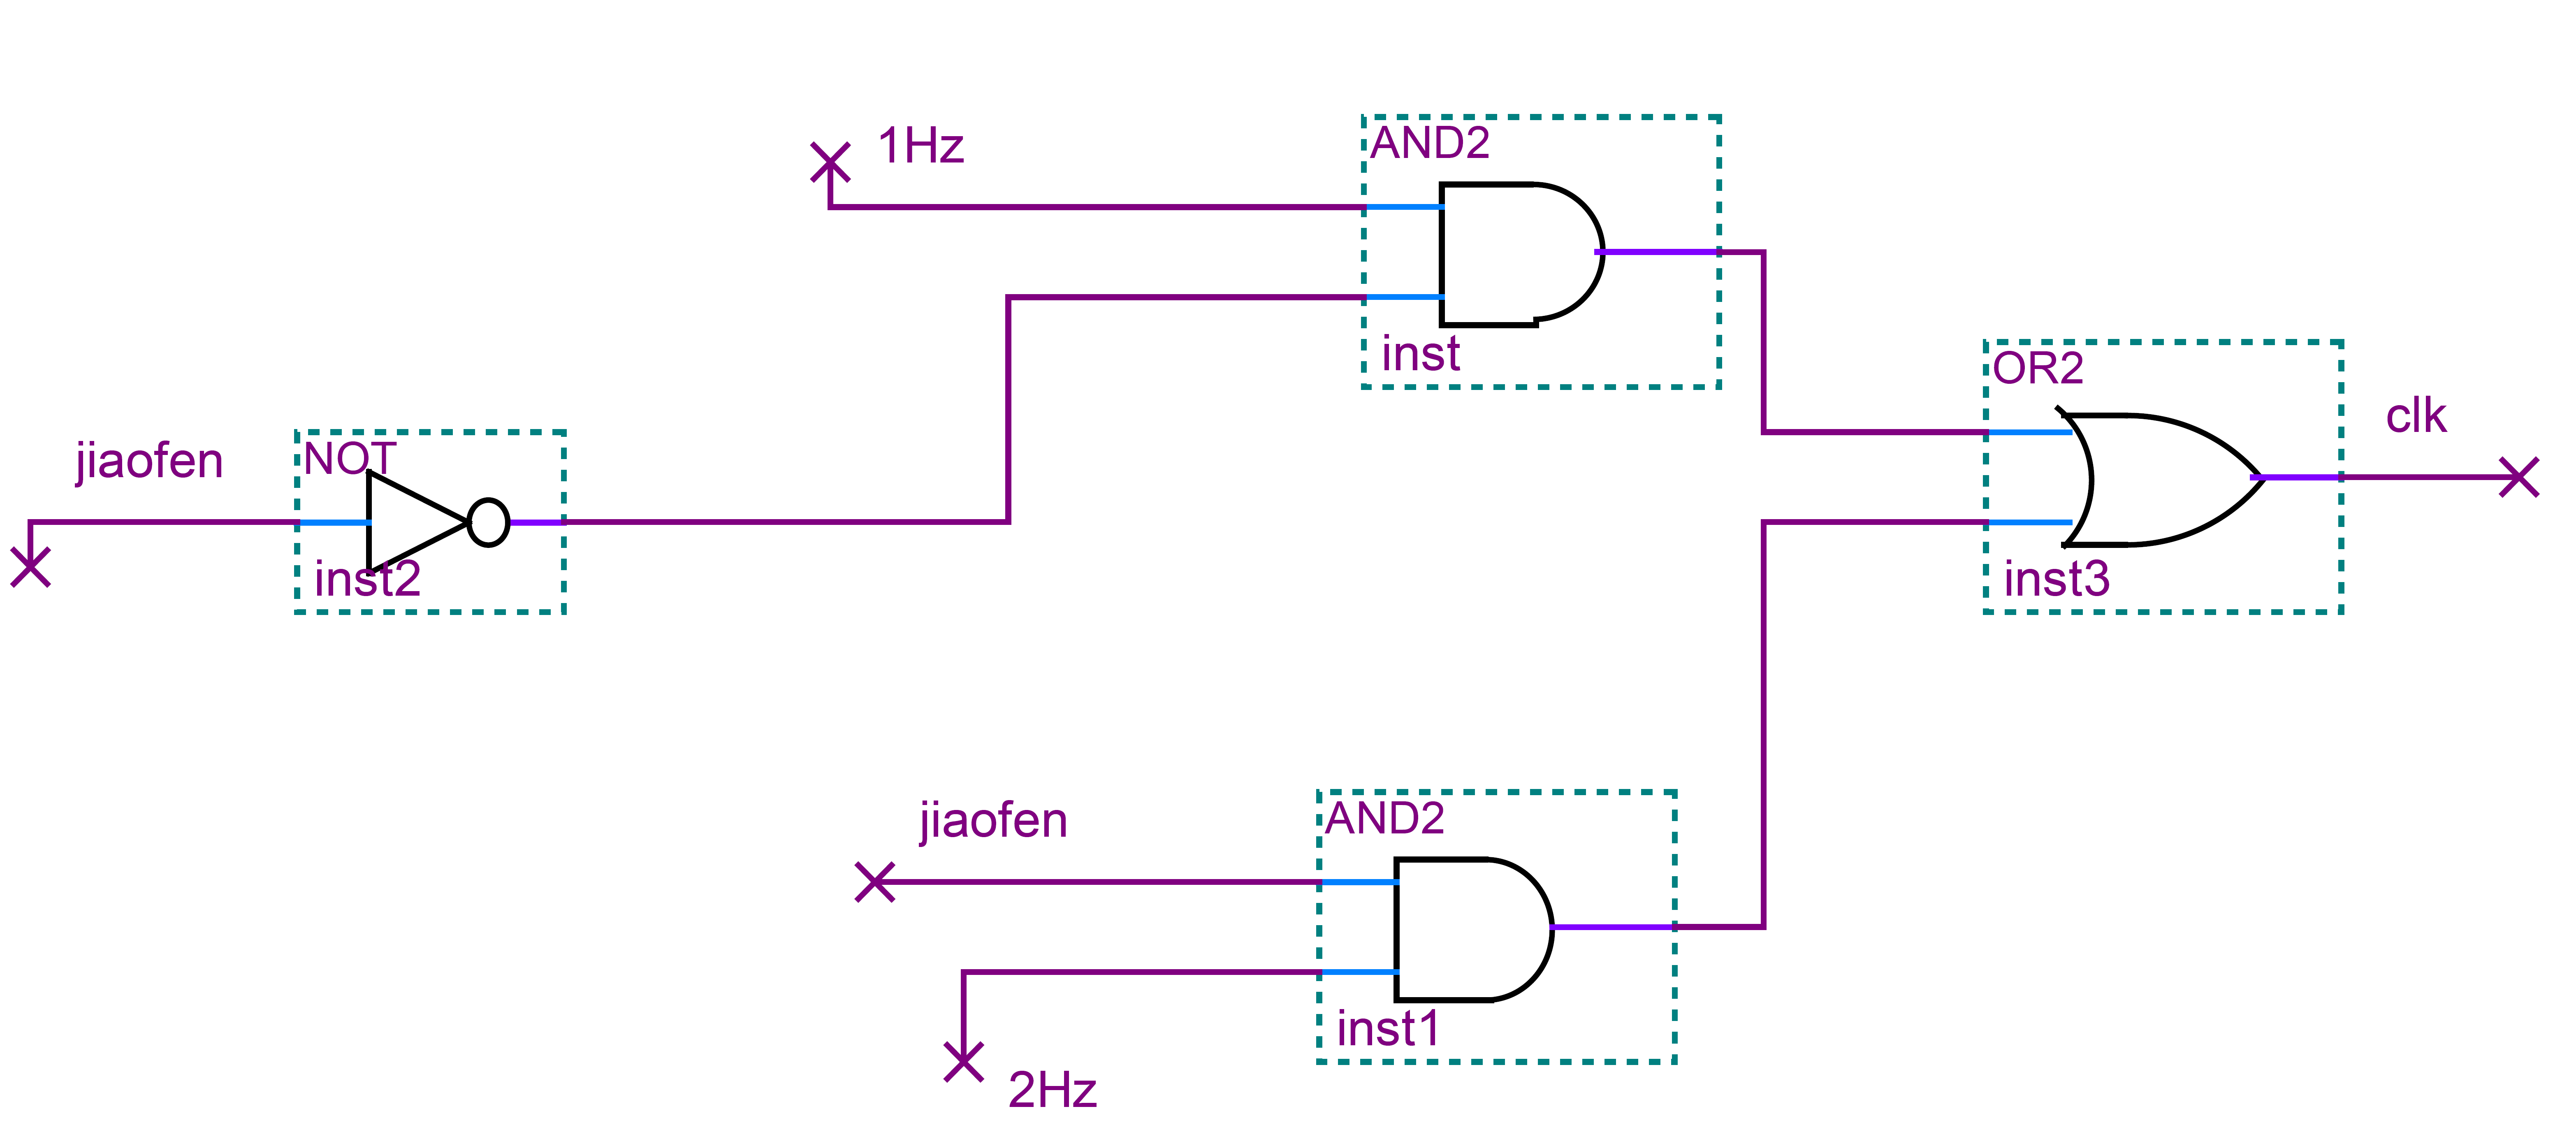
\includegraphics[width=\textwidth]{picture/jiao.png} 
	\caption{}
	\label{fig:jiao}   
\end{figure}
\begin{figure}[hp]
	\centering  
	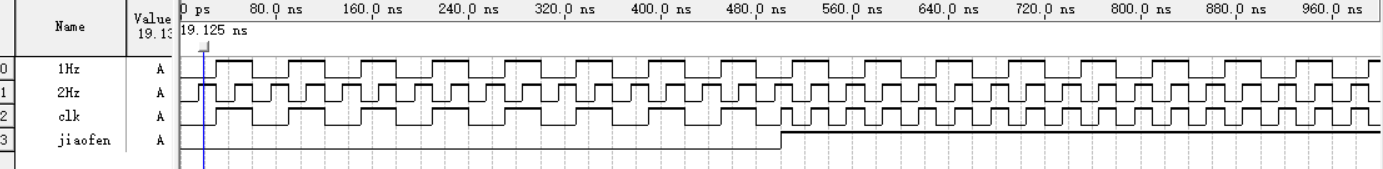
\includegraphics[width=\textwidth]{picture/fzjiaofen.png} 
	\caption{}
	\label{fig:fzjiao}   
\end{figure}
\begin{figure}[hp]
	\centering  
	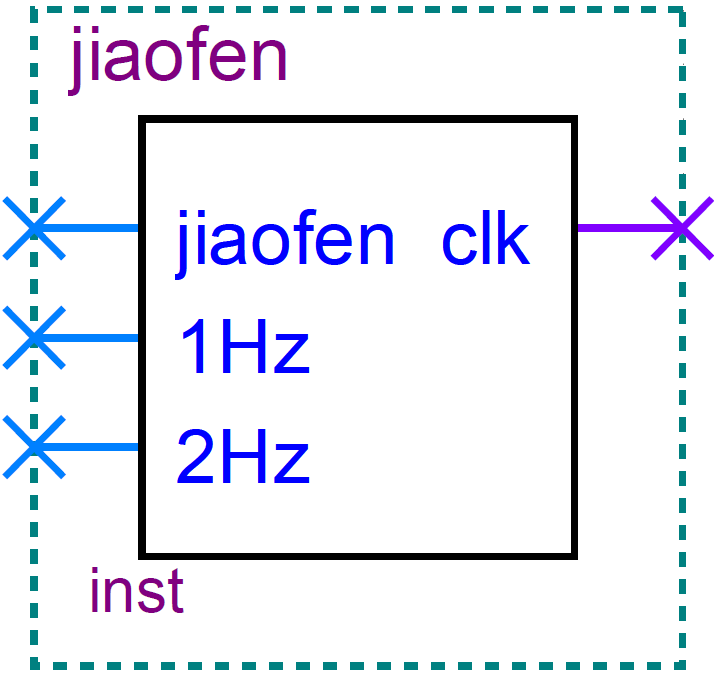
\includegraphics[width=0.3\textwidth]{picture/fenzhuangjiao.png} 
	\caption{}
	\label{fig:fengzhuangjiao}   
\end{figure}\par
\subsubsection{清零、保持模块}
\paragraph{清零}清零功能是通过控制各位计数器清零端的电平高低来实现的。因此,只需使清零开关按下时各计数器的清零端均接入低电平、清零开关断开时各清零端均接入高电平即可。\par\paragraph{保持}保持功能是通过控制计数器的使能端实现的。当$K_1=0$,通过一个非门接到使能端使计数器正常计数;当$K_1=1$时,使能端变成0,计数器停止计数,实现计时保持功能。\par而由于所有其他位的计数都依靠或直接或间接秒位的进位信号,因此使秒位使能端失效即可实现保持功能。而为了秒位的进位信号不干扰校时,任意一个校时开关开启,也同步让秒位使能失效。\par 在校时模块中,需要对使能端操作,因此在保持模块里,对应的校时开关开启,则对应的使能信号便有效。为避免干扰,低位的进位信号必须在其他校时开关均关闭时才能影响使能端,于是,这一部分的原理图见图\ref{fig:baochi},封装图见图\ref{fig:fengzhuangbaochi}。
\begin{figure}[hp]
	\centering  
	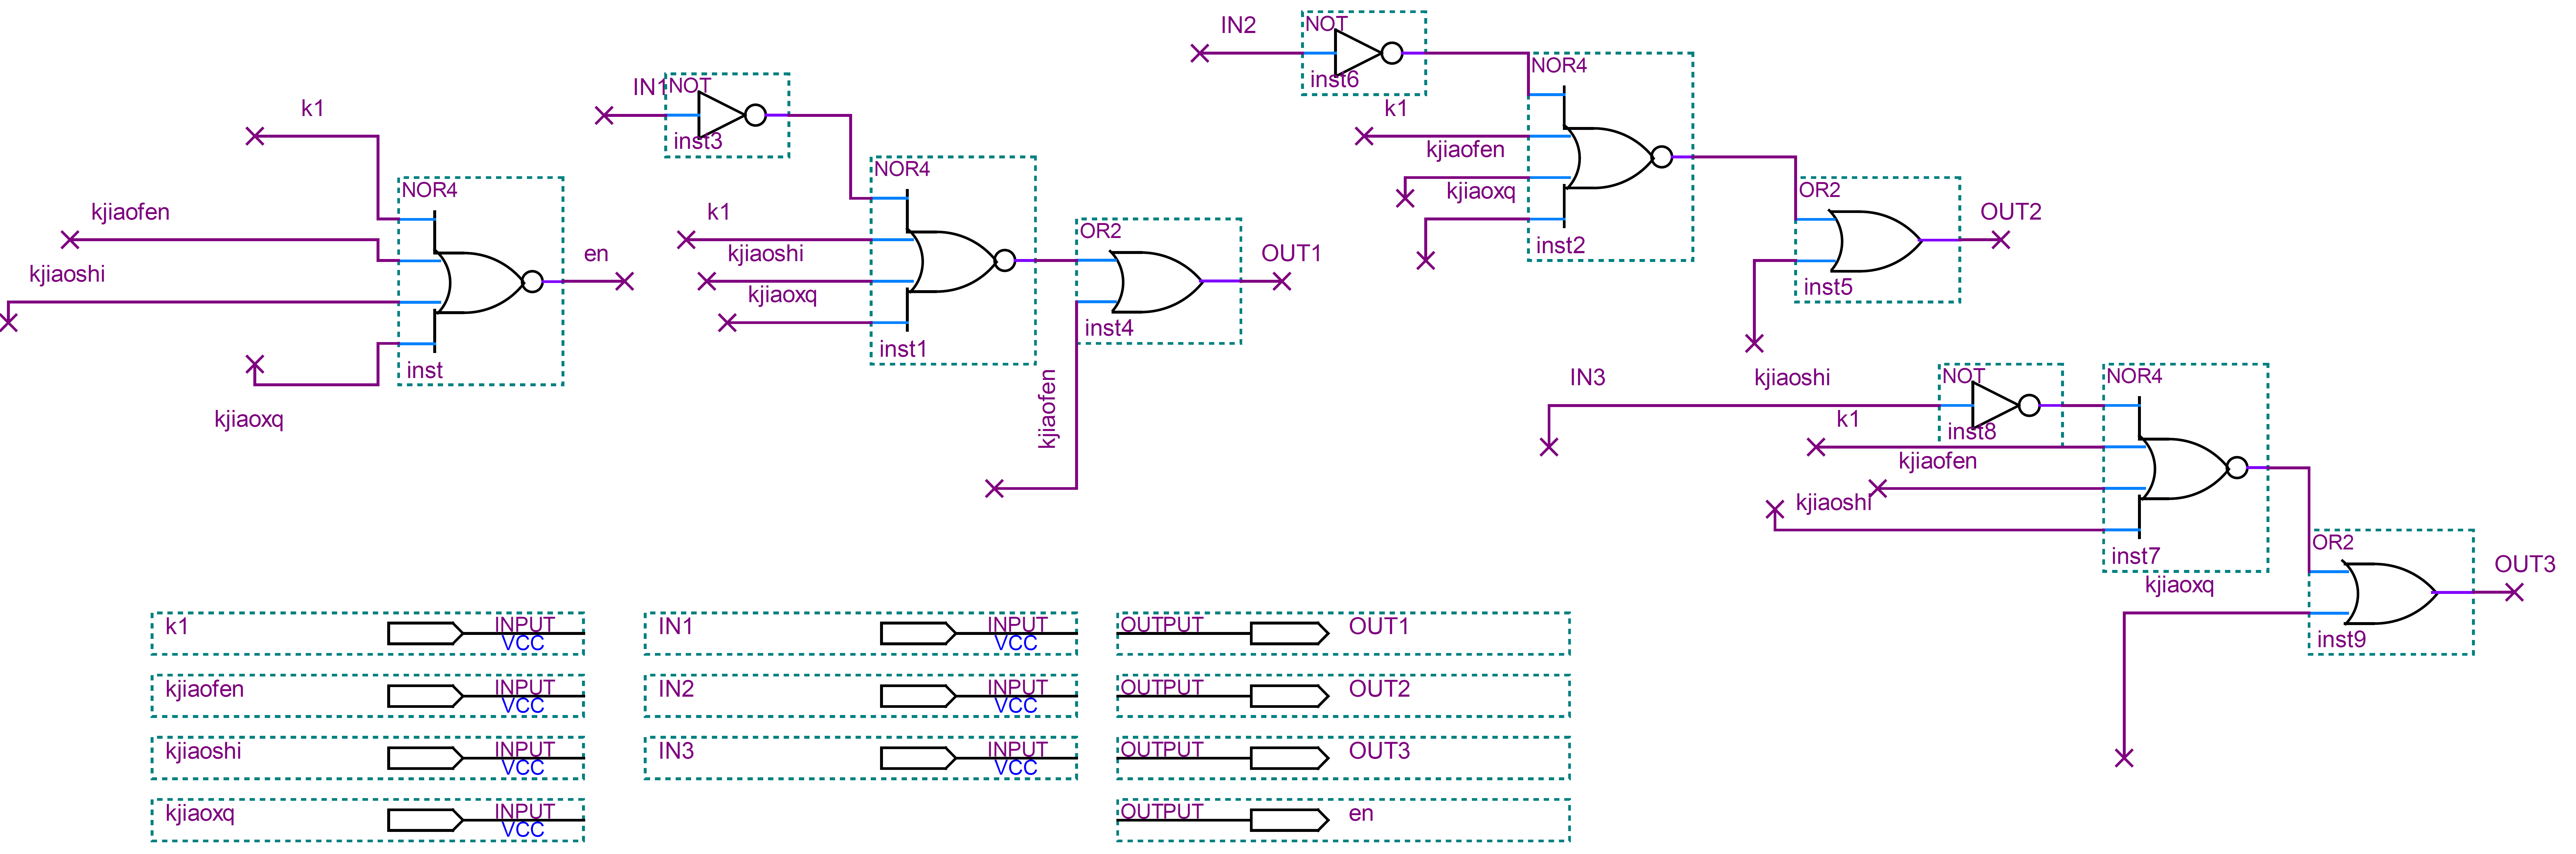
\includegraphics[width=\textwidth]{picture/baochi.png} 
	\caption{}
	\label{fig:baochi}   
\end{figure}
\begin{figure}[hp]
	\centering  
	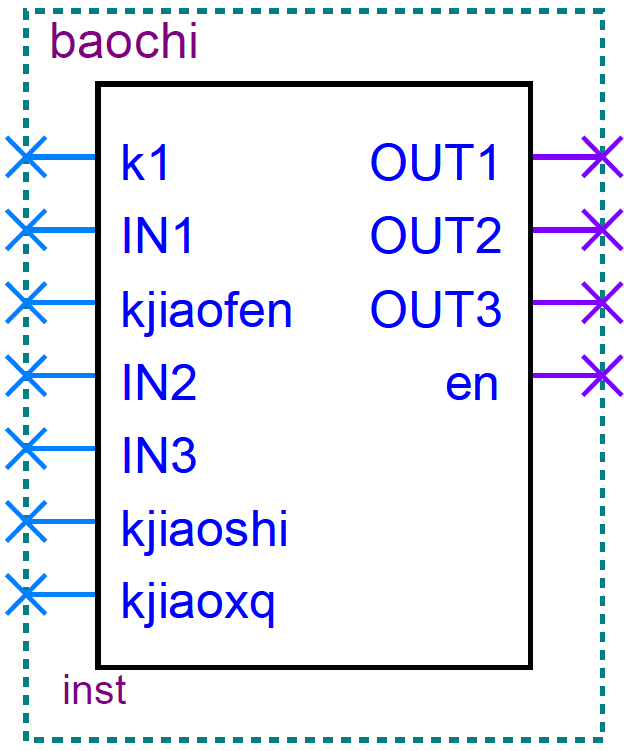
\includegraphics[width=0.3\textwidth]{picture/fenzhuangbaochi.png} 
	\caption{}
	\label{fig:fengzhuangbaochi}   
\end{figure}\par
\subsubsection{消颤模块}
由于开关的接通和关闭有可能产生毛刺,出现竞争冒险现象,所以要对所有的开关进行消颤处理。具体是通过一个D触发器对开关信号进行延时,从而得到稳定可靠的开关信号,消颤电路的原理图见图\ref{fig:xiaochan},封装图见图\ref{fig:fenzhuangxiaochan1},整个消颤模块的电路图见图\ref{fig:xiaochanjihe},封装图见图\ref{fig:fenzhuangxiaochan}。
\begin{figure}[hp]
	\centering  
	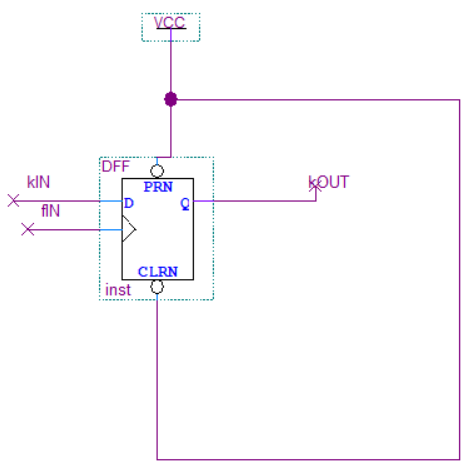
\includegraphics[width=0.5\textwidth]{picture/xiaochan.png} 
	\caption{}
	\label{fig:xiaochan}   
\end{figure}
\begin{figure}[hp]
	\centering  
	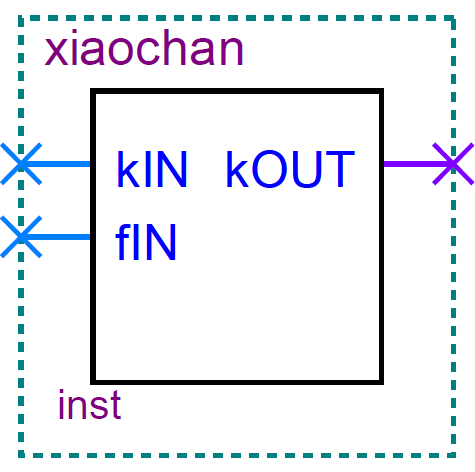
\includegraphics[width=0.3\textwidth]{picture/fenzhuangxiaochan1.png} 
	\caption{}
	\label{fig:fenzhuangxiaochan1}   
\end{figure}\par
\begin{figure}[hp]
	\centering  
	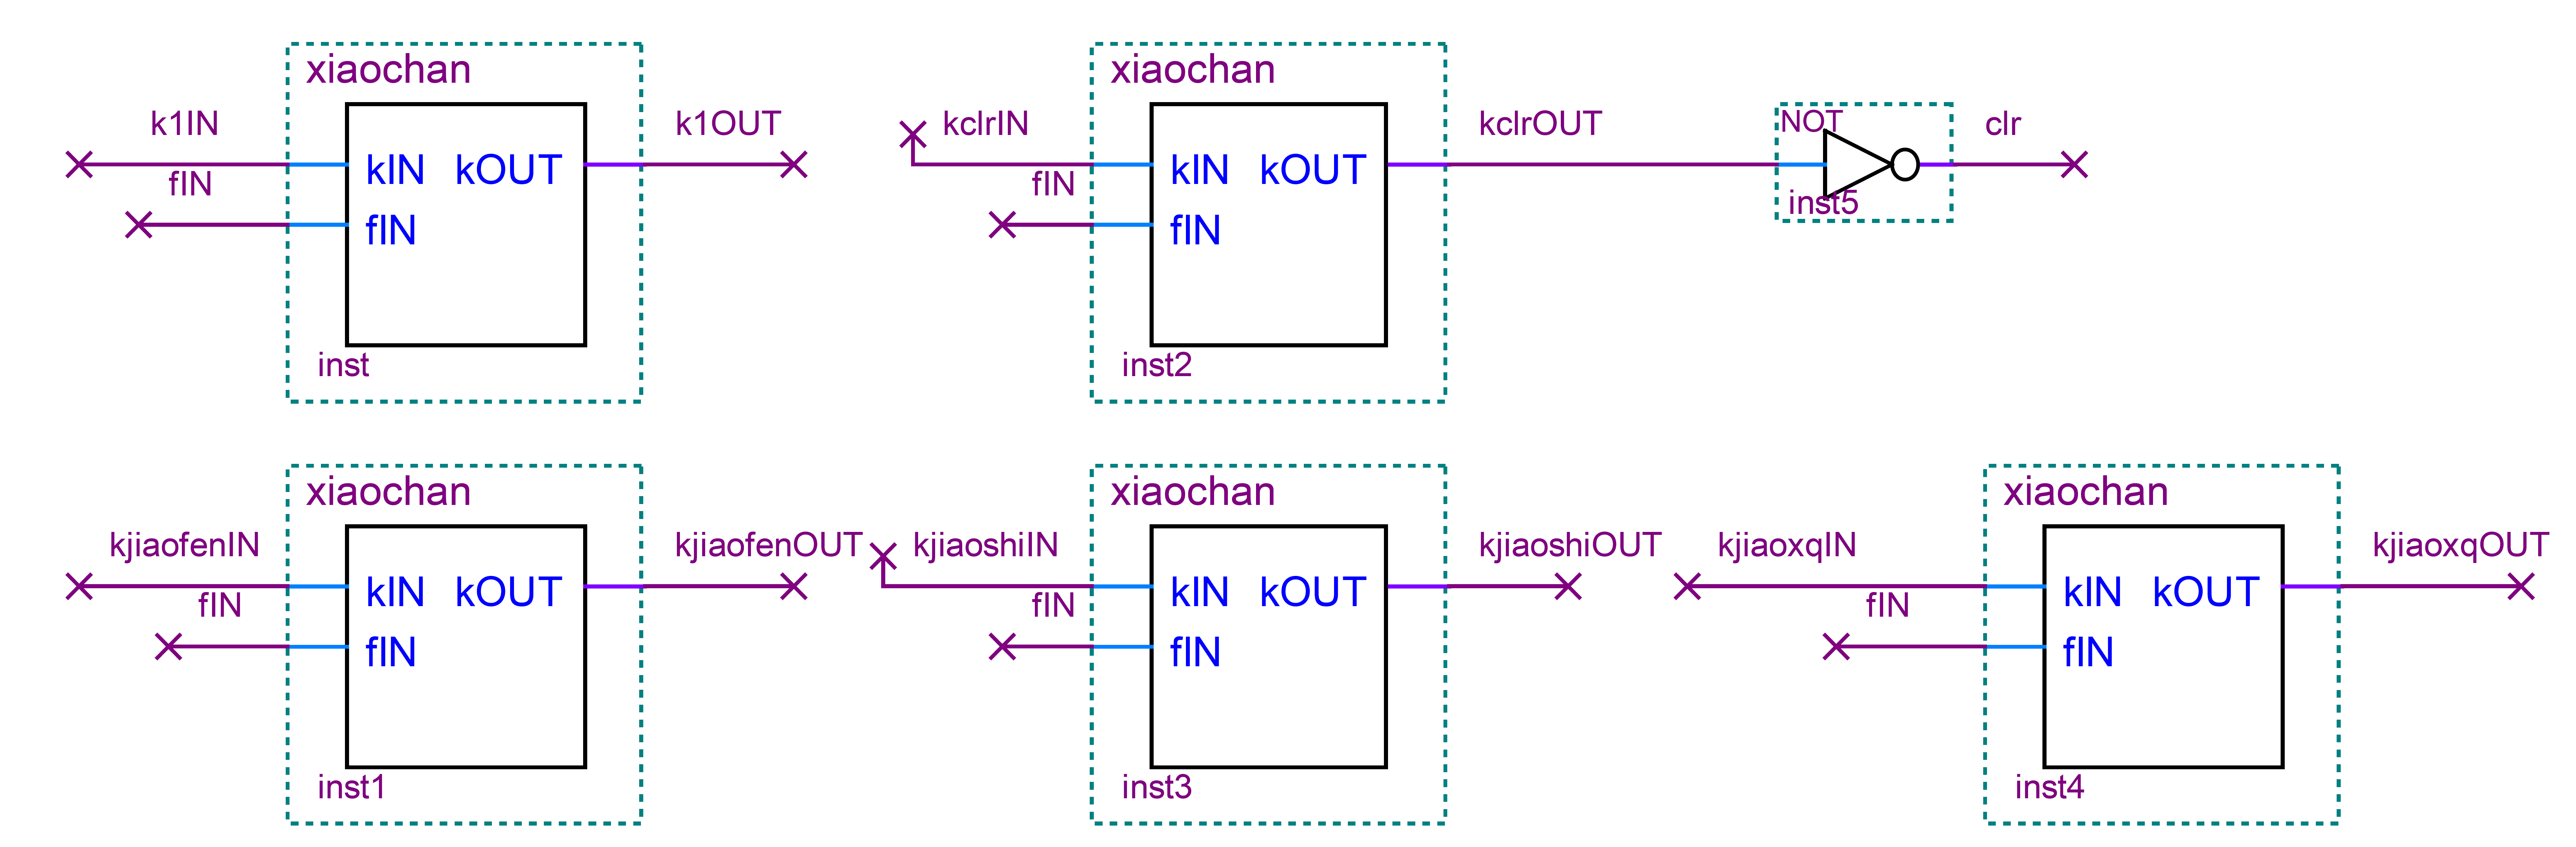
\includegraphics[width=\textwidth]{picture/xiaochanjihe.png} 
	\caption{}
	\label{fig:xiaochanjihe}   
\end{figure}
\begin{figure}[hp]
	\centering  
	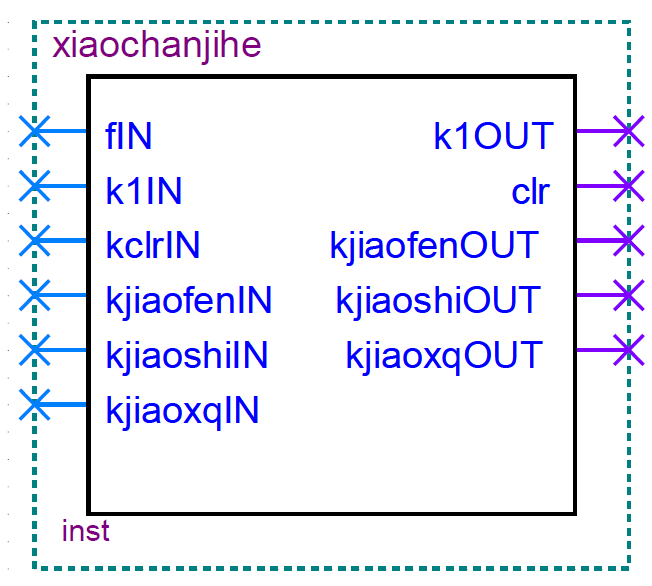
\includegraphics[width=0.3\textwidth]{picture/fenzhuangxiaochan.png} 
	\caption{}
	\label{fig:fenzhuangxiaochan}   
\end{figure}\par
\subsubsection{报时模块}
报时模块要求数字钟在 59 分 53 秒、59 分 55 秒、59 分 57 秒时低音报时,在 59 分 59 秒时高音报时,需要使用 1000Hz、500Hz 两种信号分别驱动。\par
列出各个时刻的各位输出状态见表\ref{tab:baoshi},分析报时条件。\par
\begin{table}[htbp]
  \centering
  \caption{报时输出状态}\label{tab:baoshi}
    \begin{tabular}{cccccc}
    \hline
    时刻 & 分十位 & 分个位 & 秒十位 & 秒个位 & 频率 \\
    \hline
    59分53秒 & 0101 & 1001 & 0101 & 0011 & 500Hz \\
    59分55秒 & 0101 & 1001 & 0101 & 0101 & 500Hz \\
    59分57秒 & 0101 & 1001 & 0101 & 0111 & 500Hz \\
    59分59秒 & 0101 & 1001 & 0101 & 1001 & 1kHz \\
    \hline
    \end{tabular}%
\end{table}%
经过分析,可得蜂鸣器的输入端应满足的表达式为:$$\left\{
             \begin{array}{c}
             F=F_1\cap F_2\\
             F_1=fs[3]\cap fs[1]\cap fg[4]\cap fg[1]\cap ms[3]\cap ms[1]\cap mg[1]\\
             F_2=500HZ\cap mg[2]+500Hz\cap mg[3]+1KHz\cap mg[4]
             \end{array}
\right.$$\par 原理图见图\ref{fig:baoshi},封装图见图\ref{fig:fenzhuangbaoshi}。
\begin{figure}[hp]
	\centering  
	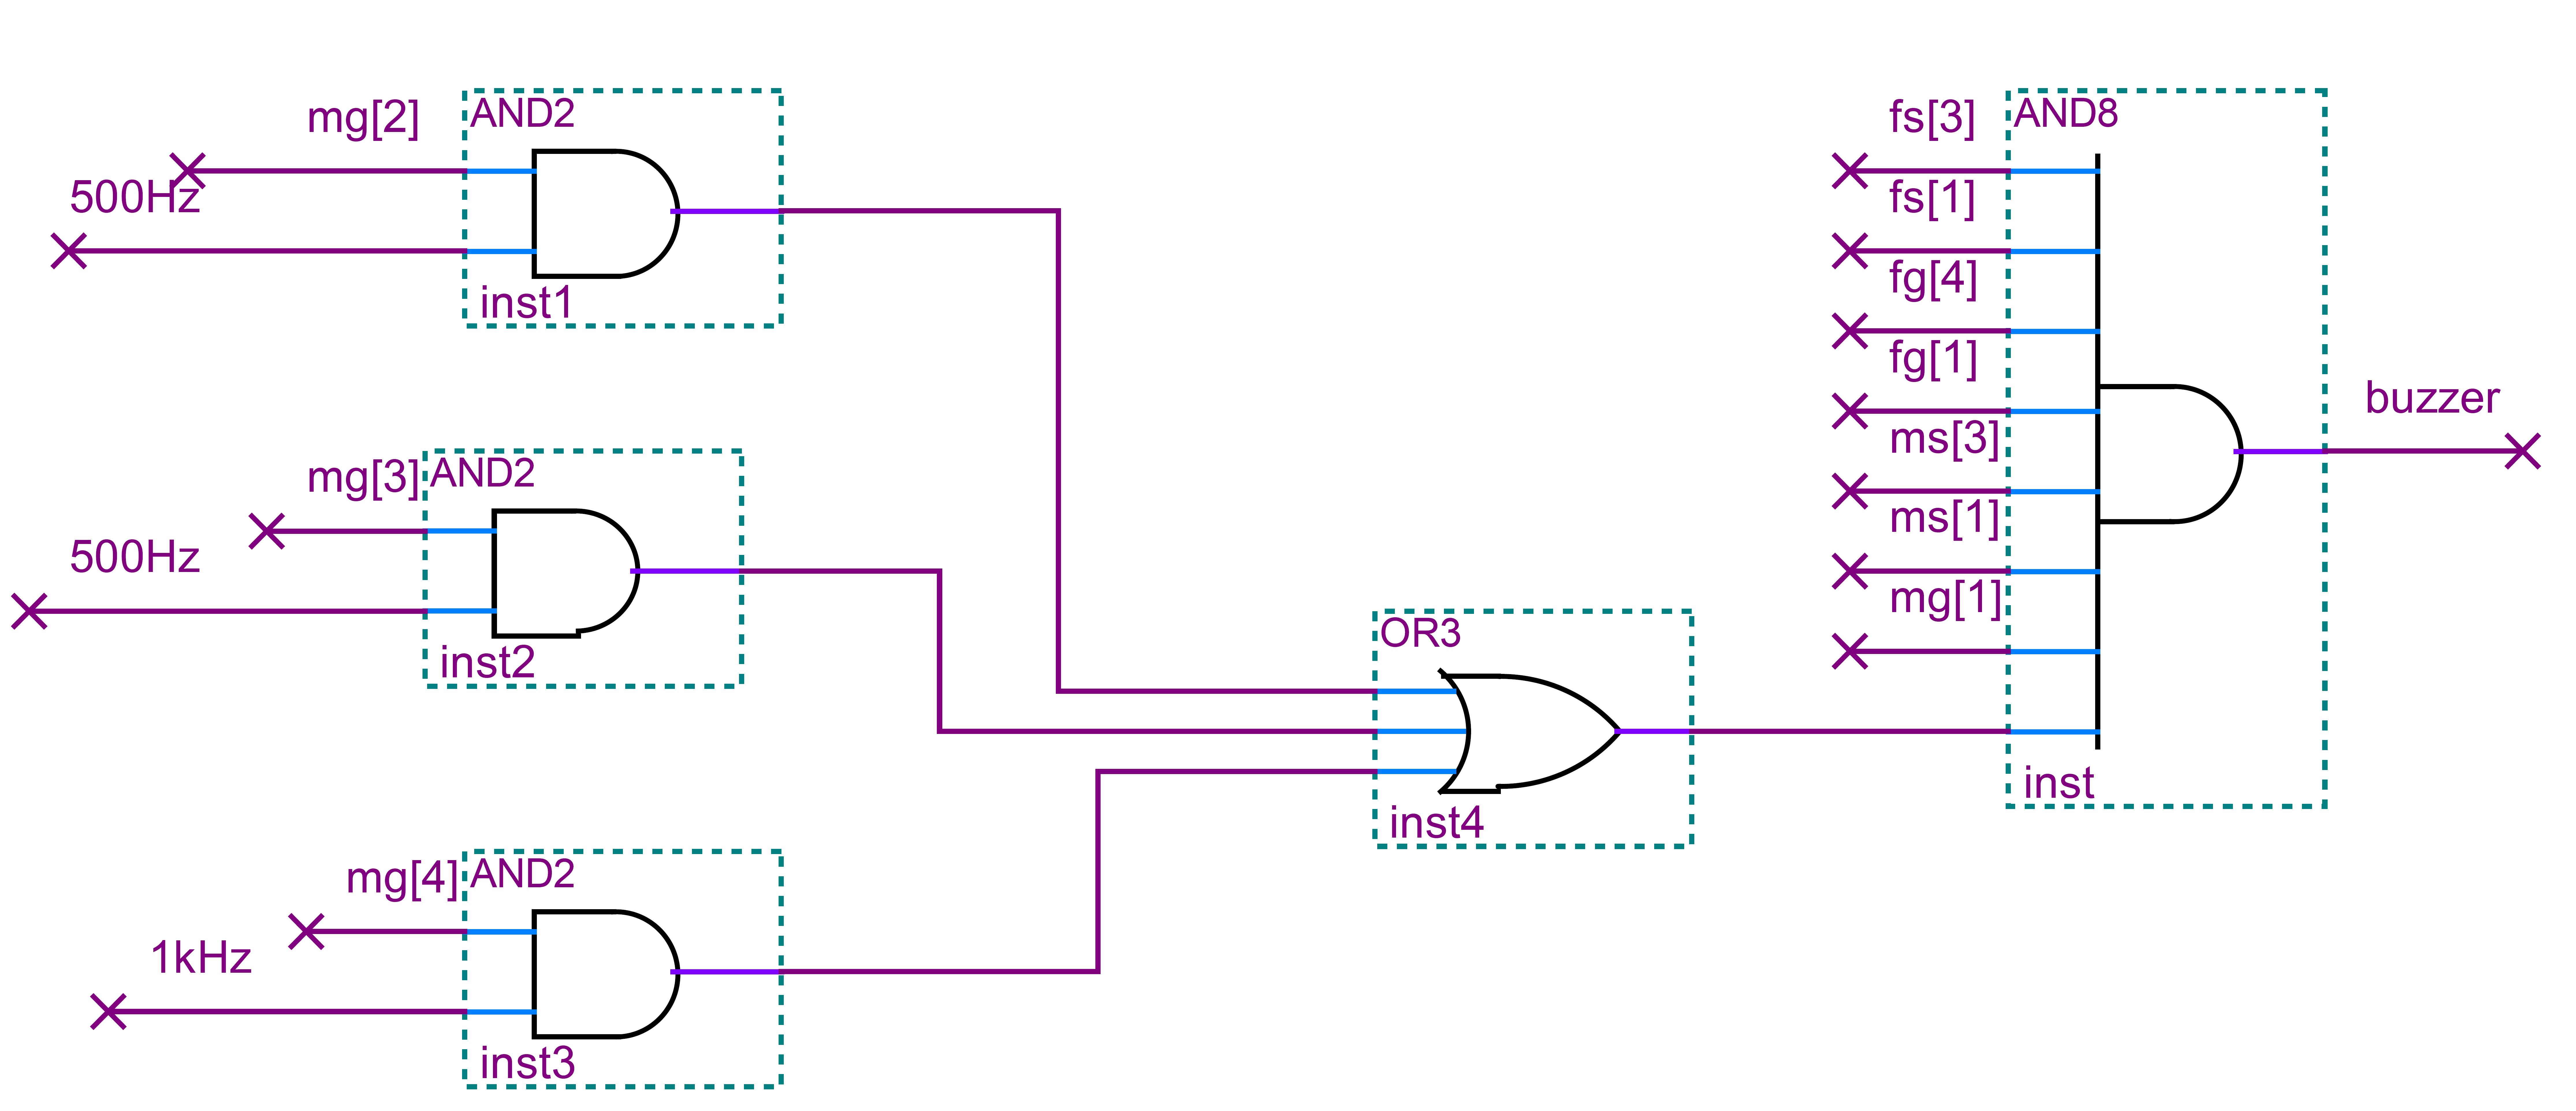
\includegraphics[width=\textwidth]{picture/baoshi.png} 
	\caption{}
	\label{fig:baoshi}   
\end{figure}
\begin{figure}[hp]
	\centering  
	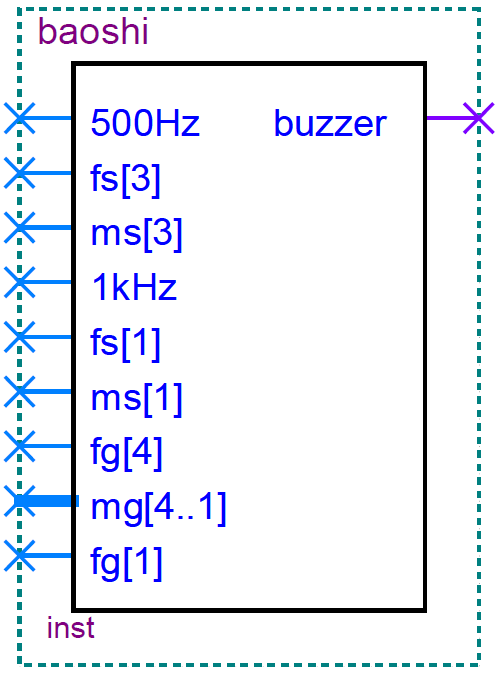
\includegraphics[width=0.3\textwidth]{picture/fenzhuangbaoshi.png} 
	\caption{}
	\label{fig:fenzhuangbaoshi}   
\end{figure}\par
\subsubsection{总计时模块}
将以上的各个模块相连,组成总的计时模块。原理图见图\ref{fig:jishi},封装图见图\ref{fig:fengzhuangjishi}。
\begin{figure}[hp]
	\centering  
	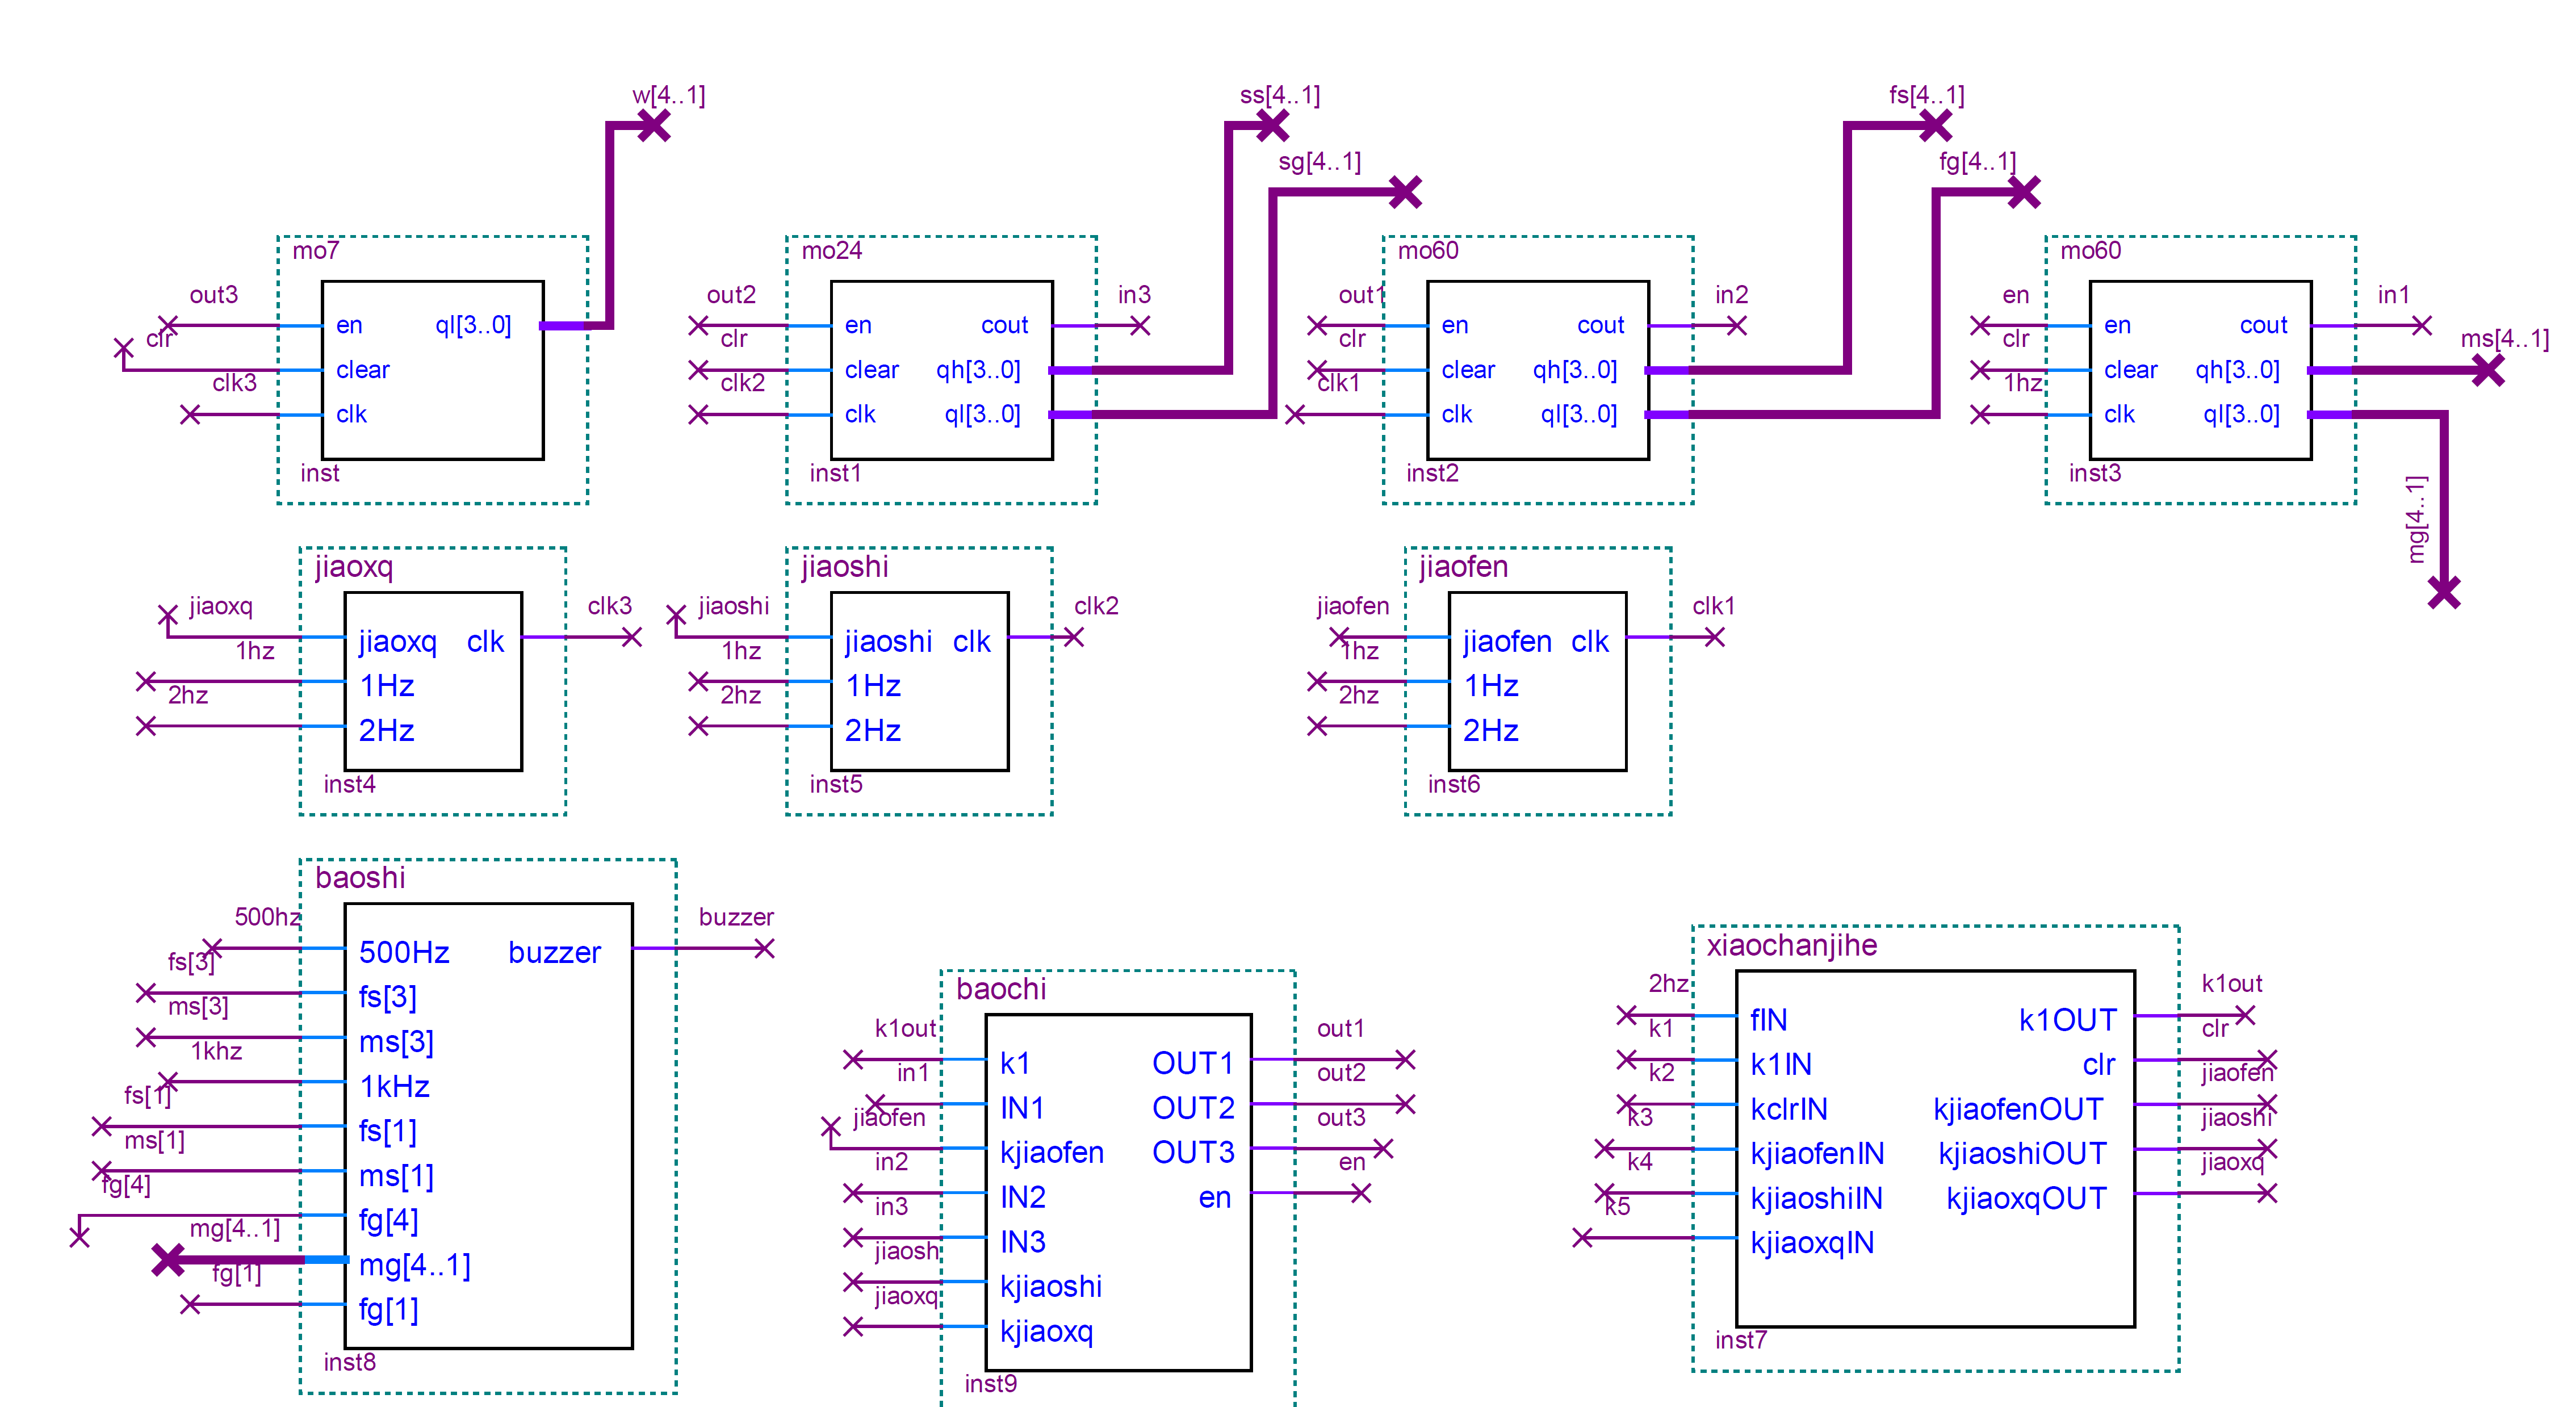
\includegraphics[width=\textwidth]{picture/jishi.png} 
	\caption{}
	\label{fig:jishi}   
\end{figure}
\begin{figure}[hp]
	\centering  
	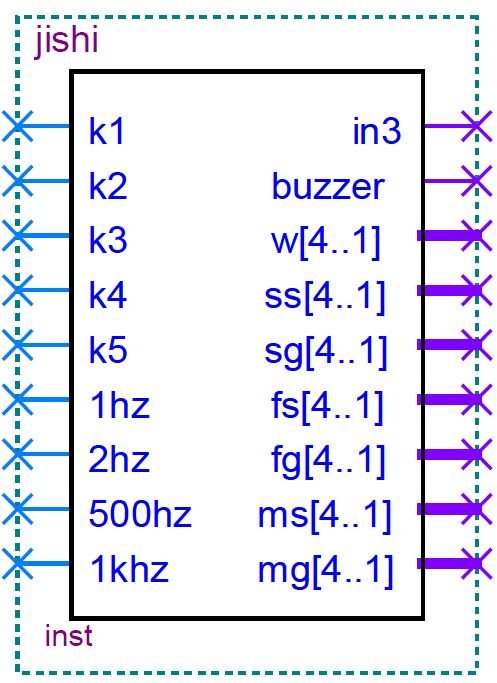
\includegraphics[width=0.3\textwidth]{picture/fenzhuangjishi.png} 
	\caption{}
	\label{fig:fengzhuangjishi}   
\end{figure}\par
\subsection{音乐模块}
这个模块可以看作我学习VHDL语言过程中的一个试验,因此与整个时钟的联系并不是十分紧密,仅仅是通过某个开关($K_6$)来控制其有无。\par
\subsubsection{音符的产生}
音乐的产生主要是通过输出不同频率的信号来控制蜂鸣器发音,通过查阅资料可以得到音符的频率关系见表\ref{tab:yinfu}\par
\begin{table}[htbp]
  \centering
  \caption{各音符对应频率}
    \begin{tabular}{cccccc}
    \hline
    音符 & 频率Hz & 音符 & 频率Hz & 音符 & 频率Hz \\
    \hline
    低1Do & 262 & 中1Do & 523 & 高1Do & 1047 \\
    低2Re & 294 & 中2Re & 587 & 高2Re & 1175 \\
    低3Mi & 330 & 中3Mi & 659 & 高3Mi & 1319 \\
    低4Fa & 349 & 中4Fa & 698 & 高4Fa & 1397 \\
    低5So & 392 & 中5So & 784 & 高5So & 1568 \\
    低6La & 440 & 中6La & 880 & 高6La & 1760 \\
    低7Si & 494 & 中7Si & 988 & 高7Si & 1967 \\
    \hline
    \end{tabular}%
  \label{tab:yinfu}%
\end{table}%
此时便不方便通过分配器产生音符了,需要通过代码实现。用VHDL语言,对时钟信号进行上升沿检测,并记录检测的数(从 0 开始计数)。如果是 N 分频,每当计数到$\frac{N}{2}-1$时将信号翻转一次,将信号输出。由此,基于表\ref{tab:yinfu}对 48MHz 进行分频。得到N的关系见表\ref{tab:yinfu2}
\begin{table}[htbp]
  \centering
  \caption{音调与计数间关系}
    \begin{tabular}{cccccc}
        \hline
    音符 & N & 音符 & N & 音符 & N \\
        \hline
    低1Do & 91742 & 中1Do & 45861 & 高1Do & 22932 \\
    低2Re & 81715 & 中2Re & 40864 & 高2Re & 20429 \\
    低3Mi & 72814 & 中3Mi & 36401 & 高3Mi & 18201 \\
    低4Fa & 68727 & 中4Fa & 34358 & 高4Fa & 17183 \\
    低5So & 61223 & 中5So & 30611 & 高5So & 15305 \\
    低6La & 54544 & 中6La & 27271 & 高6La & 13635 \\
    低7Si & 48592 & 中7Si & 24295 & 高7Si & 12148 \\
        \hline
    \end{tabular}%
  \label{tab:yinfu2}%
\end{table}%
\subsubsection{音乐模块}
得到各个音符后,设定每个音符的时间,用两只老虎的音调。再用一个变量对整首歌进行计数,这个变量也代表了时间长度,通过循环,使得整首歌不断播放。得到代码如下,封装图见\ref{fig:music}。
\begin{lstlisting}[language=VHDL]
library ieee;
use ieee.std_logic_1164.all;
ENTITY music IS
PORT(
clk : in std_logic;
beep: out std_logic
);
end music;
architecture beh of music is
type state_type is (do_l,re_l,mi_l,fa_l,sol_l,la_l,si_l,do_m,re_m,mi_m,fa_m,sol_m,la_m,si_m,do_h,re_h,mi_h,fa_h,sol_h,la_h,si_h,none);
signal counter : integer range 0 to 100000 := 0; 
signal count : integer range 0 to 99 := 0; 
signal beep_reg: std_logic;
signal clk1khz,clk4hz : std_logic;
signal note : state_type ;
begin
beep <= beep_reg;
beep_pro : process(clk)
variable cnt : integer range 0 to 100000 := 0;
begin
if clk'event and clk='1' then
if cnt < counter then
cnt := cnt + 1 ;
else
cnt := 0 ; beep_reg <= not beep_reg;
end if;
end if;
end process beep_pro;
clk1khz_pro : process(clk) 
variable cnt : integer range 0 to 23999;
begin
if clk'event and clk='1' then
if cnt = 23999 then
cnt := 0 ; clk1khz <= not clk1khz;
else 
cnt := cnt + 1;
end if;
end if;
end process clk1khz_pro;
clk4hz_pro :process(clk1khz) 
variable cnt : integer range 0 to 124 := 0;
begin
if clk1khz'event and clk1khz = '1' then
if cnt = 124 then
cnt := 0 ; clk4hz <= not clk4hz;
else
cnt := cnt + 1;
end if;
end if;
end process clk4hz_pro;
count_pro : process(clk4hz) 
begin
if clk4hz'event and clk4hz ='1' then
if count <= 66 then
count <= count + 1;
else
count <= 0;
end if;
end if;
end process count_pro;
note_pro : process(note)
begin
case note is
when do_l => counter <= 91742 ;
when re_l => counter <= 81715 ;
when mi_l => counter <= 72814 ;
when fa_l => counter <= 68727 ;
when sol_l => counter <=61223 ;
when la_l => counter <= 54544 ;
when si_l => counter <= 48592 ;
when do_m => counter <= 45861 ;
when re_m => counter <= 40864 ;
when mi_m => counter <= 36401 ;
when fa_m => counter <= 34358 ;
when sol_m => counter <=30611 ;
when la_m => counter <= 27271 ;
when si_m => counter <= 24295 ; 
when do_h => counter <= 22932 ;
when re_h => counter <= 20429 ;
when mi_h => counter <= 18201 ;
when fa_h => counter <= 17183 ;
when sol_h => counter <=15305 ;
when la_h => counter <= 13635 ;
when si_h => counter <= 12148 ;
when others => counter <= 0;
end case;
end process note_pro;
music_pro : process(count) 
begin
case count is when 0 => note <= do_m ;
when 1 => note <= do_m;
when 3 => note <= re_m;
when 5 => note <= mi_m;
when 7 => note <= do_m;
when 9 => note <= do_m;
when 11 => note <= re_m;
when 13 => note <= mi_m;
when 15 => note <= do_m;
when 17 => note <= mi_m;
when 19 => note <= fa_m;
when 21 => note <= sol_m;
when 22 => note <= sol_m;
when 23 => note <= sol_m;
when 25 => note <= mi_m;
when 27 => note <= fa_m;
when 29 => note <= sol_m;
when 30 => note <= sol_m;
when 31 => note <= sol_m ;
when 33 => note <= sol_m ;
when 34 => note <= la_m ;
when 35 => note <= sol_m ;
when 36 => note <= fa_m ;
when 37 => note <= mi_m ;
when 38 => note <= mi_m ;
when 39 => note <= do_m ;
when 40 => note <= do_m ;
when 41 => note <= sol_m;
when 42 => note <= la_m;
when 43 => note <= sol_m;
when 44 => note <= fa_m;
when 45 => note <= mi_m;
when 46 => note <= mi_m;
when 47 => note <= do_m;
when 48 => note <= do_m;
when 49 => note <= re_m;
when 50 => note <= re_m;
when 51 => note <= sol_l;
when 52 => note <= sol_l;
when 53 => note <= do_m ;
when 54 => note <= do_m ;
when 55 => note <= do_m ;
when 57 => note <= re_m;
when 58 => note <= re_m;
when 59 => note <= sol_l;
when 60 => note <= sol_l;
when 61 => note <= do_m;
when 62 => note <= do_m;
when 63 => note <= do_m;
when others => note <= none;
end case;
end process music_pro;
end beh;
\end{lstlisting} 
\begin{figure}[hp]
	\centering  
	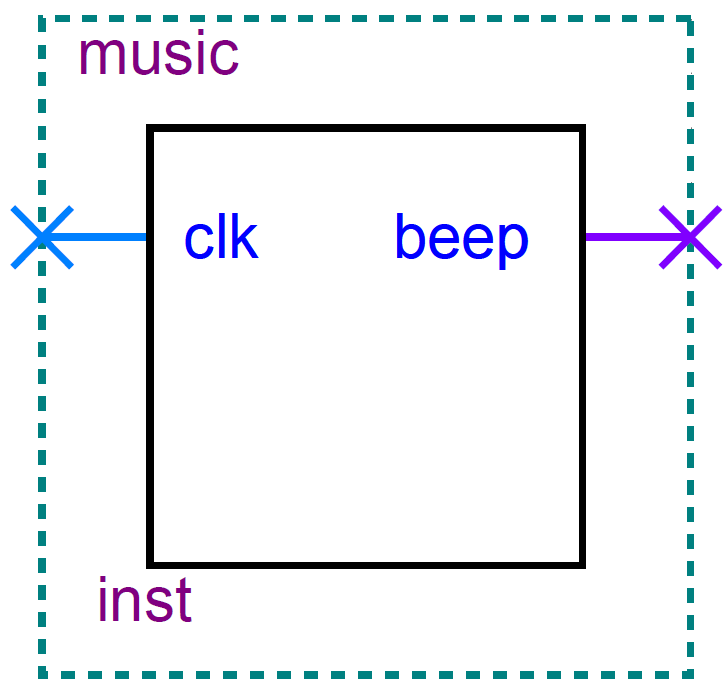
\includegraphics[width=0.3\textwidth]{picture/music.png} 
	\caption{}
	\label{fig:music}   
\end{figure}\par
\subsection{显示模块}
在数码管上的显示为动态扫描,因为同一时间只能有一个数码管有效。而当扫描的频率比较大时,就可以认为所有的数码管都是亮的。数码管有八个,而数字有七个,为了美观,在星期与时分秒中间加入了短横线。显示模块由模8模块、八选一模块、七段译码器模块、三八译码器模块组成。
\subsubsection{模8计数器}模8计数器是为了同时只让一个数码管有效,同时作为八选一选择器的输入端,选择输出的数字。其
原理与计时电路中的原理类似,代码如下,封装图见图\ref{fig:mo8}。
\begin{lstlisting}[language=VHDL]
library ieee;
use ieee.std_logic_1164.all;
use ieee.std_logic_unsigned.all;
ENTITY mo8 IS 
 PORT
(
en  :IN  std_logic;
clk  :IN  std_logic;
q :buffer std_logic_vector(2 downto 0)
);
END mo8;
ARCHITECTURE beh OF mo8 IS
BEGIN
PROCESS(clk)
BEGIN
IF(clk'EVENT and clk='1')THEN
if(en='1')then
q<=q+1;
end if;
end if;
END PROCESS;
END beh;
\end{lstlisting}\par
\begin{figure}[hp]
	\centering  
	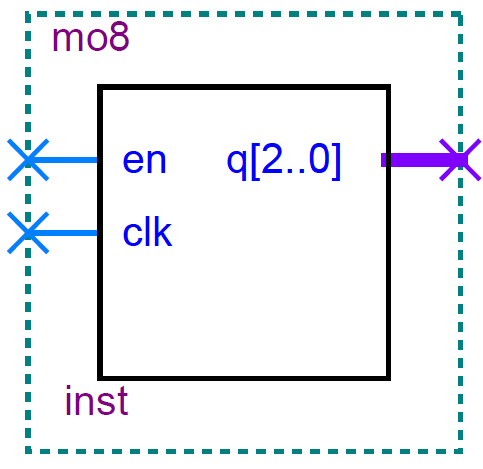
\includegraphics[width=0.3\textwidth]{picture/mo8.png} 
	\caption{}
	\label{fig:mo8}   
\end{figure}
\subsubsection{八选一}八选一用来选择当前有效的数码管应该显示的数字,有星期、短横线、时十位、时个位、分十位、分个位、十位、秒个位,这八种状态。其中短横线用1111来代替,而在之后的七段译码器中,将1111译为数码管中只有 g 段亮的短横线。代码如下,封装图见图\ref{fig:8t1}。
\begin{lstlisting}[language=VHDL]
library ieee;
use ieee.std_logic_1164.all;
use ieee.std_logic_unsigned.all;
entity chose8to1 is
port(wl,hh,hl,fh,fl,mh,ml:in std_logic_vector(3 downto 0);
sel:in std_logic_vector(2 downto 0);
q:out std_logic_vector(3 downto 0)); 
end chose8to1;
architecture chose of chose8to1 is
begin
process(sel,wl,hh,hl,fh,fl,mh,ml)
begin
case sel is
when"000"=>q<=wl;--week
when"001"=>q<="1111";--short line,to devide week and times
when"010"=>q<=hh;--shiwei of hour
when"011"=>q<=hl;--gewei of hour
when"100"=>q<=fh;--shiwei of minite
when"101"=>q<=fl;--gewei of minite
when"110"=>q<=mh;--shiwei of seconds
when"111"=>q<=ml;--gewei of seconds
when others=>q<="0000";-- don't care
end case;
end process;
end chose;
\end{lstlisting}
\begin{figure}[hp]
	\centering  
	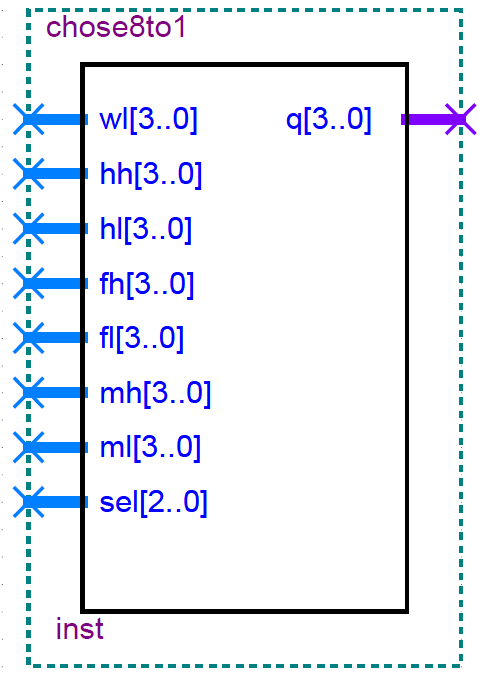
\includegraphics[width=0.3\textwidth]{picture/8t1.png} 
	\caption{}
	\label{fig:8t1}   
\end{figure}
\subsubsection{3线-8线译码器}将计数器输出的三位数据译码成八个状态,作为数据分配器使用,控制数码管有效与否。代码如下,封装图见图\ref{fig:3t8}。
\begin{lstlisting}[language=VHDL]
library ieee;
use ieee.std_logic_1164.all;
use ieee.std_logic_unsigned.all;
entity translate3to8 is
port(a:in std_logic_vector(2 downto 0);
y:out std_logic_vector(7 downto 0));
end translate3to8;
architecture translate of translate3to8 is
begin
process(a)
begin
case a is
when"000"=>y<="01111111";--wk
when"001"=>y<="10111111";--short line
when"010"=>y<="11011111";
when"011"=>y<="11101111";
when"100"=>y<="11110111";
when"101"=>y<="11111011";
when"110"=>y<="11111101";
when"111"=>y<="11111110";
when others=>y<="11111111";--don't chose
end case;
end process;
end translate;
\end{lstlisting}
\begin{figure}[hp]
	\centering  
	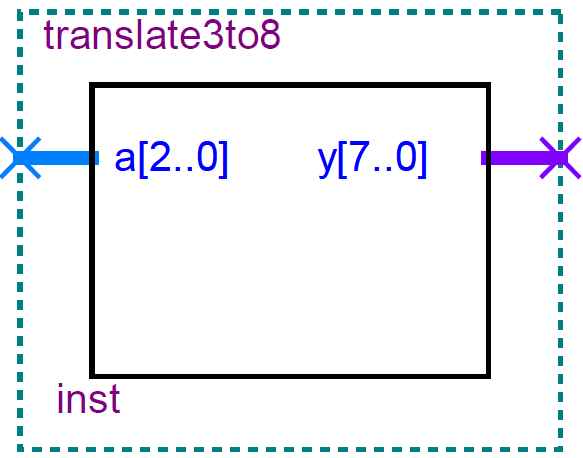
\includegraphics[width=0.3\textwidth]{picture/3t8.png} 
	\caption{}
	\label{fig:3t8}   
\end{figure}
\subsubsection{七段译码器}将二进制的数字译码为数码管中 a、b、c、d、e、f、g 段的显示情况,能直观地显示出数字来。我们所用的数码管为共阳。其中,转换方案见表\ref{tab:yima}。由此,得到代码如下,封装图见图\ref{fig:yima}
\begin{table}[hp]
  \centering
  \caption{数码管译码方案}
    \begin{tabular}{cccccccc}
    \hline
字型 & a & b & c & d & e & f & g \\
\hline
0  & 0 & 0 & 0 & 0 & 0 & 0 & 1 \\
1  & 1 & 0 & 0 & 1 & 1 & 1 & 1 \\
2  & 0 & 0 & 1 & 0 & 0 & 1 & 0 \\
3  & 0 & 0 & 0 & 0 & 1 & 1 & 0 \\
4  & 0 & 1 & 0 & 0 & 1 & 0 & 0 \\
5  & 0 & 1 & 0 & 0 & 1 & 0 & 0 \\
6  & 0 & 1 & 0 & 0 & 0 & 0 & 0 \\
7  & 0 & 0 & 0 & 1 & 1 & 1 & 1 \\
8  & 0 & 0 & 0 & 0 & 0 & 0 & 0 \\
9  & 0 & 0 & 0 & 0 & 1 & 0 & 0\\
    \hline
    \end{tabular}%
  \label{tab:yima}%
\end{table}
\begin{lstlisting}[language=VHDL]
library ieee;
use ieee.std_logic_1164.all;
use ieee.std_logic_unsigned.all;
entity yimaqi is
port(a:in std_logic_vector(3 downto 0);
y:out std_logic_vector(6 downto 0));
end yimaqi;
architecture yima of yimaqi is
begin
process(a)
begin
case a is--0 means light;1 means dark
when"0000"=>y<="1000000";
when"0001"=>y<="1111001";
when"0010"=>y<="0100100";
when"0011"=>y<="0110000";
when"0100"=>y<="0011001";
when"0101"=>y<="0010010";
when"0110"=>y<="0000010";
when"0111"=>y<="1111000";
when"1000"=>y<="0000000";
when"1001"=>y<="0010000";
when"1111"=>y<="0111111";
when others=>y<="1111111";--no words
end case;
end process;
end yima;
\end{lstlisting}
\begin{figure}[hp]
	\centering  
	\includegraphics[width=0.3\textwidth]{picture/yima.png} 
	\caption{}
	\label{fig:yima}   
\end{figure}
\subsubsection{显示模块}
将以上几个部分组合,得到显示模块如图\ref{fig:xianshi},封装图见图\ref{fig:fengzhuangxianshi}。
\begin{figure}[hp]
	\centering  
	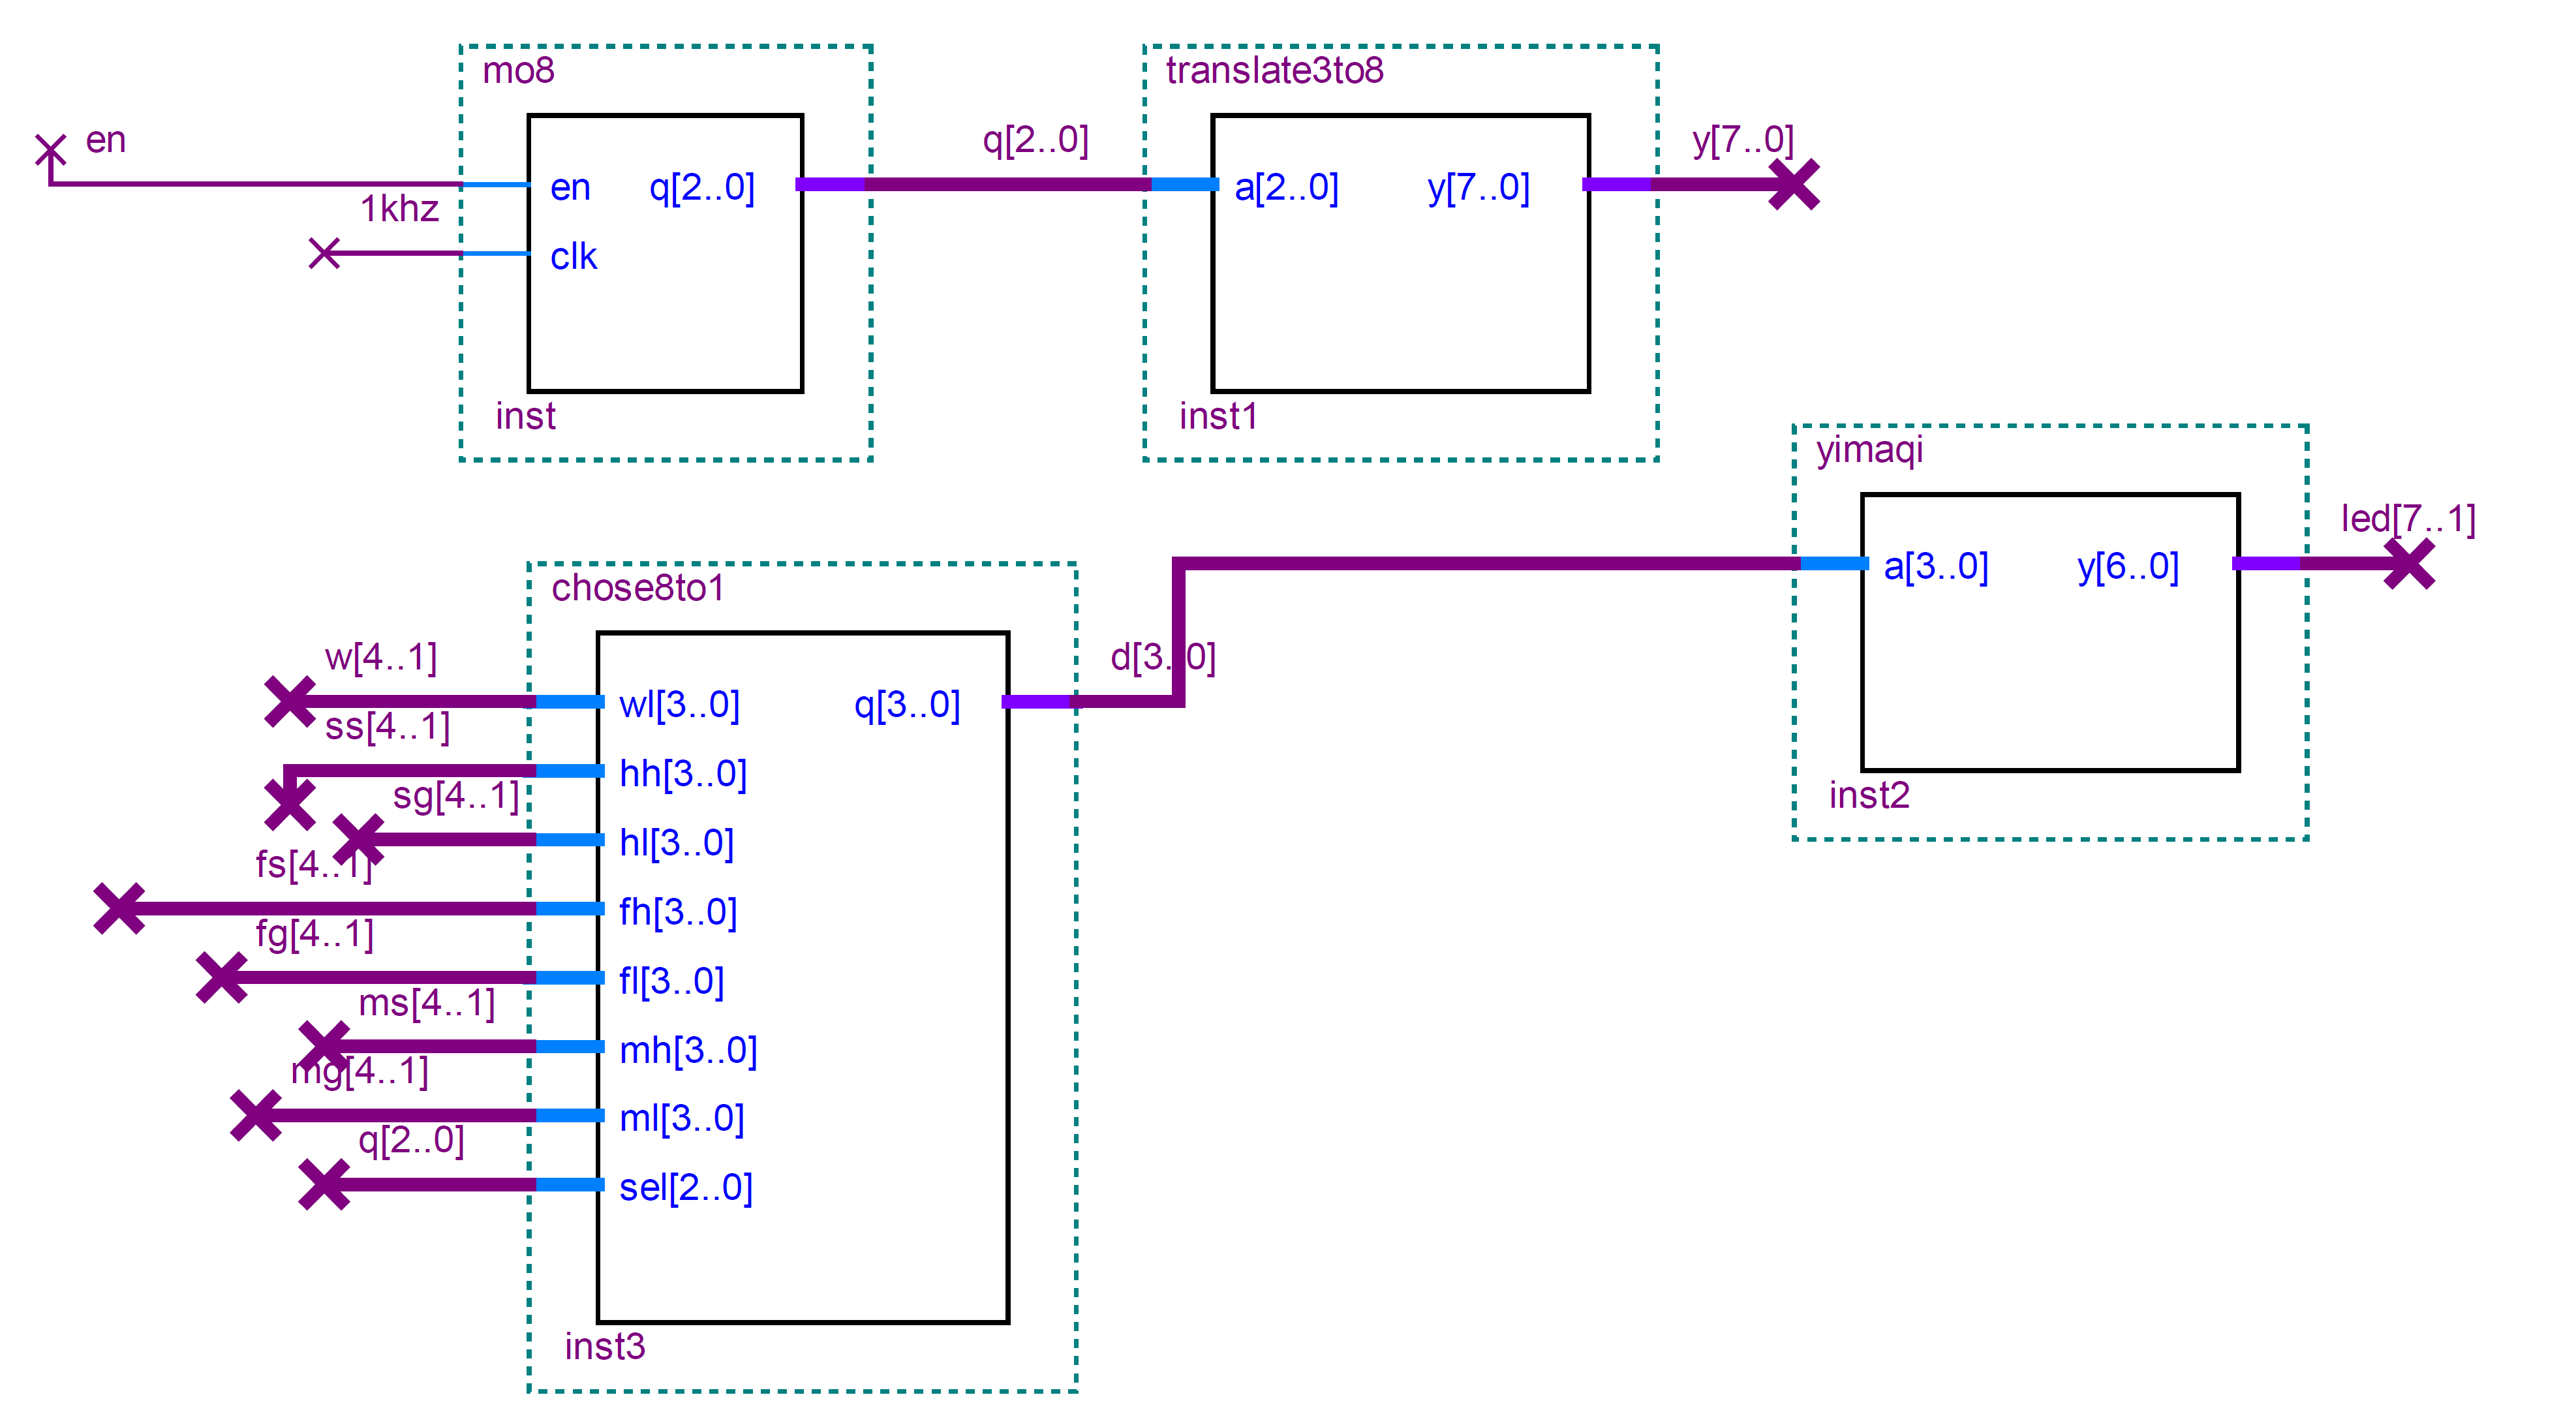
\includegraphics[width=\textwidth]{picture/xianshi.png} 
	\caption{}
	\label{fig:xianshi}   
\end{figure}
\begin{figure}[hp]
	\centering  
	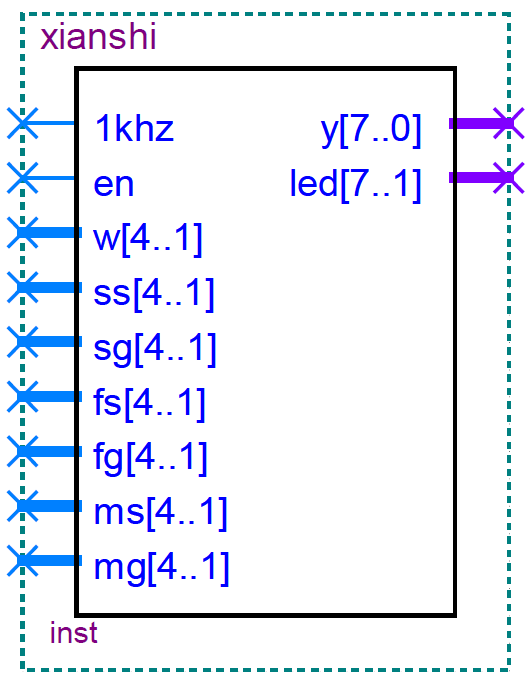
\includegraphics[width=0.3\textwidth]{picture/fenzhuangxianshi.png} 
	\caption{}
	\label{fig:fengzhuangxianshi}   
\end{figure}\par
\subsection{万年历模块}
要实现万年历,即是对日、月、年的显示,其中日有28、29、30、31四种情况。而年有润年平年之分。在我的时钟中,是通过每四年输出一个信号来判断润年与否的,因此对于整百年的情况,这里无法判断。
\subsubsection{日计数}
根据年、月的不同,日会有28、29、30、31四种情况,因此引入一个2位的judge信号,根据judge确定进制。juege为00时,采用28进制;juege为01时,采用29进制;juege为10时,采用30进制;juege为11时,采用31进制。VHDL代码如下,仿真情况见图\ref{fig:fzday1}$\sim$\ref{fig:fzday4},封装图见\ref{fig:fengzhuangday}。
\begin{lstlisting}[language=VHDL]
library ieee;
use ieee.std_logic_1164.all;
use ieee.std_logic_unsigned.all;
ENTITY day IS 
 PORT
(
clear:IN  std_logic;
judge :IN std_logic_vector(1 downto 0);--judge how many days
clk :IN  std_logic;
dh :buffer std_logic_vector(3 downto 0);
dl :buffer std_logic_vector(3 downto 0);
rco : OUT std_logic;
 en   :IN  std_logic
);
END day;
ARCHITECTURE beh OF day IS
BEGIN
PROCESS(clk,judge,clear)
BEGIN
IF(clk'EVENT and clk='1')THEN
IF(en='1')then
IF(clear='0')THEN
dh<="0000";dl<="0000";
else
case judge is
when"00"=>--28
if(dh=2 and dl=8)then
rco<='1';dh<="0000";dl<="0001";
else if(dl=9)then
dh<=dh+1;dl<="0000";rco<='0';
else rco<='0';dl<=dl+1;
end if;
end if;
when"01"=>--29
if(dh=2 and dl=9)then
rco<='1';dh<="0000";dl<="0001";
else if(dl=9)then
dh<=dh+1;dl<="0000";rco<='0';
else rco<='0';dl<=dl+1;
end if;
end if;
when"10"=>--30
if(dh=3 and dl=0)then
rco<='1';dh<="0000";dl<="0001";
else if(dl=9)then
dh<=dh+1;dl<="0000";rco<='0';
else rco<='0';dl<=dl+1;
end if;
end if;
when others =>--31
if(dh=3 and dl=1)then
rco<='1';dh<="0000";dl<="0001";
else if(dl=9)then
dh<=dh+1;dl<="0000";rco<='0';
else rco<='0';dl<=dl+1;
end if;
end if;
end case;
end if;
end IF;
end if;
END PROCESS;
END beh;
\end{lstlisting}
\begin{figure}[hp]
	\centering  
	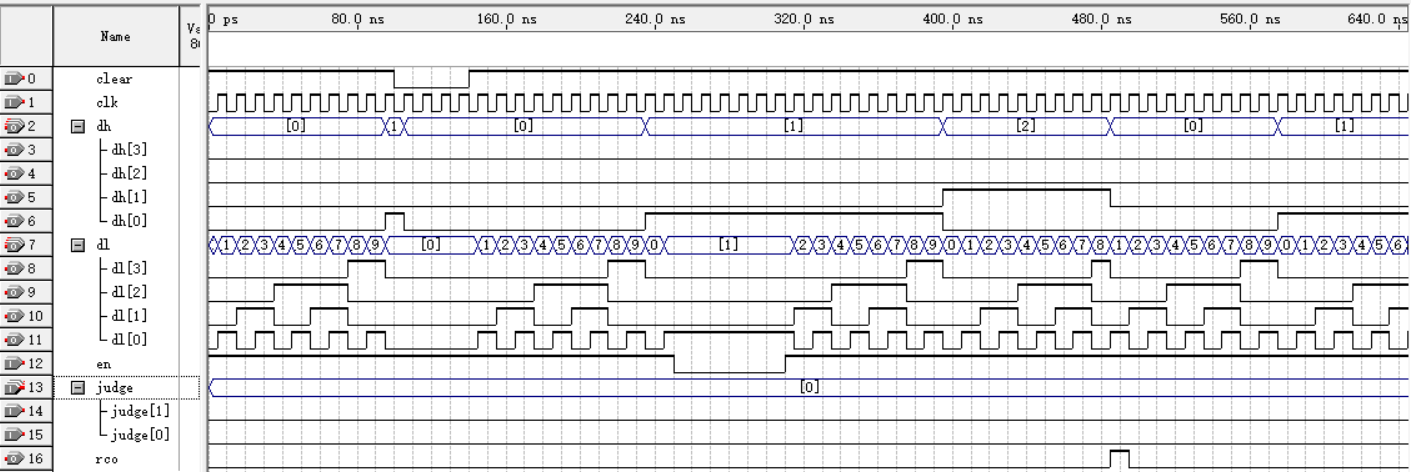
\includegraphics[width=\textwidth]{picture/fzday00.png} 
	\caption{}
	\label{fig:fzday1}   
\end{figure}
\begin{figure}[hp]
	\centering  
	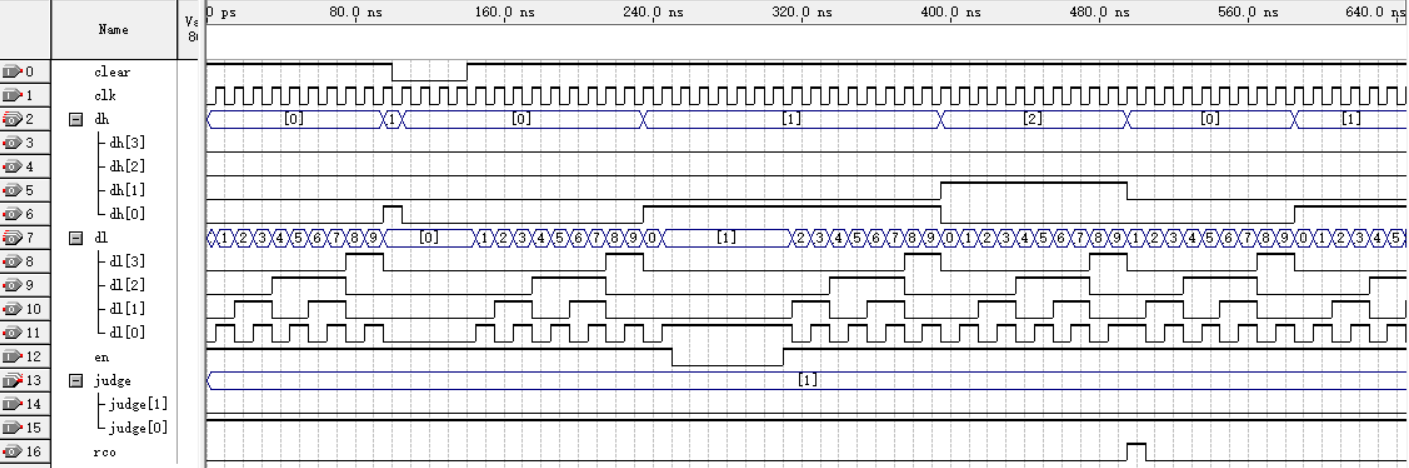
\includegraphics[width=\textwidth]{picture/fzday01.png} 
	\caption{}
	\label{fig:fzday2}   
\end{figure}
\begin{figure}[hp]
	\centering  
	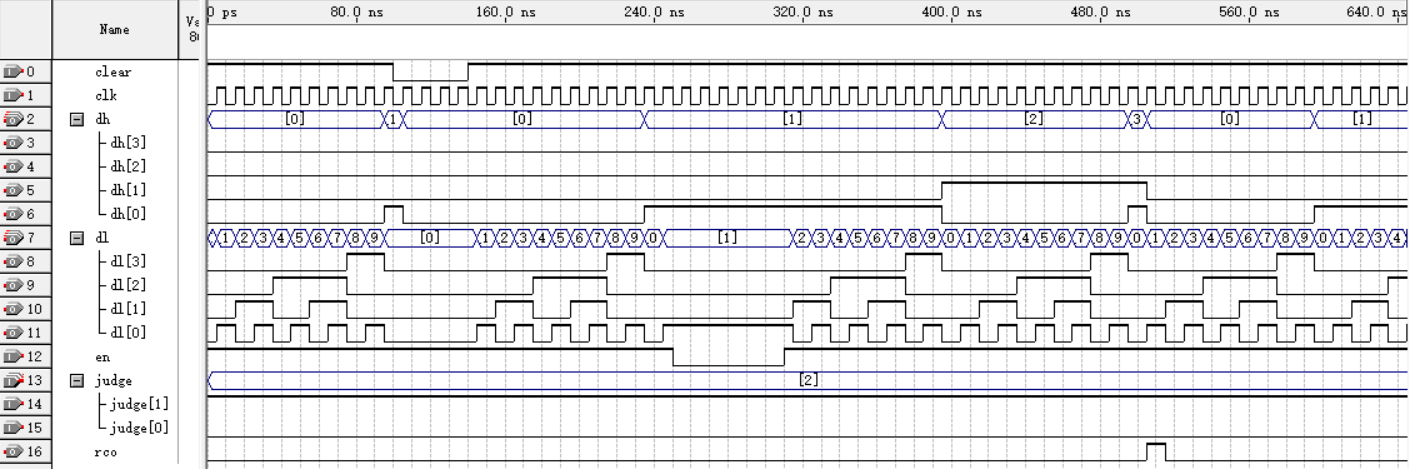
\includegraphics[width=\textwidth]{picture/fzday10.png} 
	\caption{}
	\label{fig:fzday3}   
\end{figure}
\begin{figure}[hp]
	\centering  
	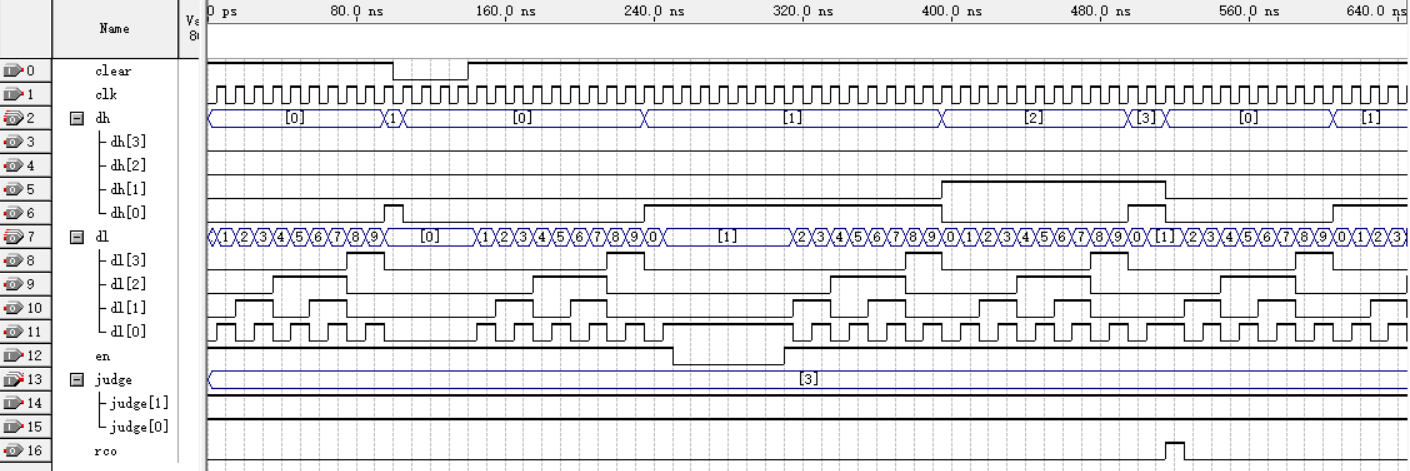
\includegraphics[width=\textwidth]{picture/fzday11.png} 
	\caption{}
	\label{fig:fzday4}   
\end{figure}
\begin{figure}[hp]
	\centering  
	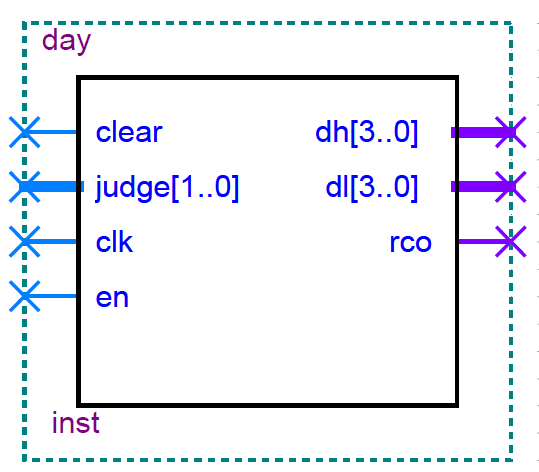
\includegraphics[width=0.3\textwidth]{picture/dayfz.png} 
	\caption{}
	\label{fig:fengzhuangday}   
\end{figure}
\subsubsection{月计数}
对于月而言,就是一个模12计数器,VHDL代码如下,仿真情况见图\ref{fig:fzmonth},封装图见\ref{fig:fengzhuangmonth}。
\begin{lstlisting}[language=VHDL]
library ieee;
use ieee.std_logic_1164.all;
use ieee.std_logic_unsigned.all;
ENTITY month IS 
 PORT
( en   :IN  std_logic;
clear:IN  std_logic;--when 0,output is always 0
clk  :IN  std_logic;
rco :out  std_logic;--jinwei output
mh :buffer std_logic_vector(3 downto 0);--shiwei output
ml :buffer std_logic_vector(3 downto 0)
);--gewei output
END month;
ARCHITECTURE beh OF month IS
BEGIN
rco<='1'when(mh="0001"and ml="0010"and en='1')else'0'; 

PROCESS(clk,clear)
BEGIN
IF(clear='0')THEN
mh<="0000";
ml<="0000";
ELSIF(clk'EVENT AND clk='1')THEN
 if(en='1')then
 if((ml=9) or (ml=2 and mh=1))then
 if(ml=2 and mh=1)then
ml<="0001";
mh<="0000";
else ml<="0000";
mh<="0001";
end if;
 else ml<=ml+1;
 end if;
  end if;
END IF;
END PROCESS;
END beh;
\end{lstlisting}
\begin{figure}[hp]
	\centering  
	\includegraphics[width=\textwidth]{picture/fzmonth.png} 
	\caption{}
	\label{fig:fzmonth}   
\end{figure}
\begin{figure}[hp]
	\centering  
	\includegraphics[width=0.3\textwidth]{picture/monthfz.png} 
	\caption{}
	\label{fig:fengzhuangmonth}   
\end{figure}
\subsubsection{年计数}
对于年而言,需要输出一个信号,表明本年是否是润年,这里采用的方法是每四年输出一个run信号,judge可由此判断是否为润年。VHDL代码如下,仿真情况见图\ref{fig:fzyear},封装图见\ref{fig:fengzhuangyear}。
\begin{lstlisting}[language=VHDL]
library ieee;
use ieee.std_logic_1164.all;
use ieee.std_logic_unsigned.all;
ENTITY year IS 
 PORT
(
clear:IN  std_logic;
clk :IN  std_logic;
run :OUT  std_logic;
r :buffer  std_logic_vector(1 downto 0);
y1 :buffer std_logic_vector(3 downto 0);
y2 :buffer std_logic_vector(3 downto 0);
y3 :buffer std_logic_vector(3 downto 0);
y4 :buffer std_logic_vector(3 downto 0);
en :IN  std_logic
);
END year;
ARCHITECTURE beh OF year IS
BEGIN
PROCESS(clk,clear)
BEGIN

IF(clk'EVENT and clk='1')THEN
IF(clear='0')THEN
y1<="0000";y2<="0000";y3<="0000";y4<="0000";r<="00";
else
if(en='1')then
if(y4=9)then
y4<="0000";y3<=y3+1;
else if(y3=9)then
y3<="0000";y2<=y2+1;
else if(y2=9)then
y2<="0000";y1<=y1+1;
else if(y1=9)then
y1<="0000";
else y4<=y4+1;
end if;
end if;
end if;
end if;
if(r=3)then
run<='1';r<="00";
else r<=r+1;run<='0';
end if;
end IF;
end if;
end if;
END PROCESS;
END beh;
\end{lstlisting}
\begin{figure}[hp]
	\centering  
	\includegraphics[width=\textwidth]{picture/fzyear.png} 
	\caption{}
	\label{fig:fzyear}   
\end{figure}
\begin{figure}[hp]
	\centering  
	\includegraphics[width=0.3\textwidth]{picture/yearfz.png} 
	\caption{}
	\label{fig:fengzhuangyear}   
\end{figure}
\subsubsection{日进制判断信号judge}
judge需要通过当前年份(run)来判断是否为润年,结合月最终给出每个月的具体日数,VHDL代码如下,仿真情况见图\ref{fig:fzjud},封装图见\ref{fig:fengzhuangjud}。
\begin{lstlisting}[language=VHDL]
library ieee;
use ieee.std_logic_1164.all;
use ieee.std_logic_unsigned.all;
ENTITY judge IS 
 PORT
(
run :IN std_logic;
mh :IN std_logic_vector(3 downto 0);
ml :IN std_logic_vector(3 downto 0);
j :buffer std_logic_vector(1 downto 0)
);
END judge;
ARCHITECTURE beh OF judge IS
BEGIN
PROCESS(run,ml,mh)
BEGIN
IF(ml=1 or ml=3 or ml=5 or ml=7 or ml=8 or (ml=0 and mh=1) or (ml=2 and mh=1 ) )THEN
j<="11";
else if(ml=4 or ml=6 or ml=9 or (ml=1 and mh=1 ))then
j<="10";
else if((ml=2 and mh=0) and run='1')then
j<="01";
else j<="00";
end if;
end if;
end IF;
END PROCESS;
END beh;
\end{lstlisting}
\begin{figure}[hp]
	\centering  
	\includegraphics[width=\textwidth]{picture/fzjude.png} 
	\caption{}
	\label{fig:fzjud}   
\end{figure}
\begin{figure}[hp]
	\centering  
	\includegraphics[width=0.3\textwidth]{picture/judfz.png} 
	\caption{}
	\label{fig:fengzhuangjud}   
\end{figure}
\subsubsection{万年历模块}
将以上计数器组合成万年历模块如图\ref{fig:nianli},仿真波形大致情况见图\ref{fig:fangzhennianli},封装图见图\ref{fig:fengzhuangnianli}。
\begin{figure}[hp]
	\centering  
	\includegraphics[width=\textwidth]{picture/nianli.png} 
	\caption{}
	\label{fig:nianli}   
\end{figure}
\begin{figure}[hp]
	\centering  
	\includegraphics[width=\textwidth]{picture/fznianli.png} 
	\caption{}
	\label{fig:fangzhennianli}   
\end{figure}
\begin{figure}[hp]
	\centering  
	\includegraphics[width=0.3\textwidth]{picture/nianlifz.png} 
	\caption{}
	\label{fig:fengzhuangnianli}   
\end{figure}
\section{多功能数字时钟总电路}
将以上几个模块相连,借助$IPM\_MUX$实现显示复用,借助74139实现开关复用,多功能数字时钟总电路如图\ref{fig:all-2}。
\begin{figure}[hp]
	\centering  
	\includegraphics[width=\textwidth]{picture/all-all.png} 
	\caption{}
	\label{fig:all-2}   
\end{figure}
\begin{lstlisting}[language=VHDL]
\end{lstlisting}
\section{调试、仿真、编程下载}
电路设计完成后,还要对已完成的电路图保存后进行编译,检查有无出错的地方,比如线路定义出错,引脚未定义等软件能检查出来的错误,这是最基本的检查,只能检查出一些语法运用的错误。\par然后还要对其进行波形仿真验证,来检查电路设计的正确与否,直至调试的仿真图完全正确为止,仿真得到的波形图在各个模块的论证时已经给出。 \par
波形仿真完成后,就要下载到实验箱上进行验收。下载方法比较繁琐,通常要设置一些程序的初始值、使能端等,但这是必须的一步,否则可能烧坏实验箱
上的某些原件,造成较大的损失。\par

将编译好的程序管脚分配,然后下载到实验系统中进行调试和验证。其中管脚分配如图\ref{fig:pins}。
\begin{figure}[hp]
	\centering  
	\includegraphics[width=\textwidth]{picture/pins.png} 
	\caption{}
	\label{fig:pins}   
\end{figure}
\section{ 结论}
运行后可实现的功能有:
\begin{enumerate}[1、]
\item 开关全部置0时,进行星期、时、分、秒计时,由7个数码管分别显示星期、时、分、秒,有整点报时功能;
\item $K_1$是系统的使能开关($K_1=0$正常工作,$K_1=1$时钟
保持不变);
\item $K_2$是系统的清零开关($K_2=0$正常工作,$K_2=1$时钟
的所有位,包括万年历部分,全部清零);
\item $K_3$是系统的校分开关($K_3=0$正常工作,$K_3=1$时可
以快速校分);
\item $K_4$是系统的校时开关($K_4=0$正常工作,$K_4=1$时可
以快速校时);
\item 而$K_4,K_5$合起来进行校星期,当$K_4,K_5$均为1时,可以快速校星期;
\item $K_5$是万年历显示开关($K_5=0$显示星期、时、分、秒,$K_5=1$时显示年-月-日 );
\item $K_6$是系统的校日开关($K_6=0$正常工作,$K_6=1$时可
以快速校日);
\item $K_7$是系统的校月开关($K_7=0$正常工作,$K_7=1$时可
以快速校月);
\item 而$K_6,K_7$合起来进行校年,当$K_6,K_7$均为1时,可以快速校年;
\item $K_8$是音乐开关($K_8=0$无音乐,$K_8=1$时循环播放两只老虎的音乐);
\item  界面更直观,星期显示,则星期与时分秒间用短横线间隔显示;万年历显示,则年、月、日间用短横线间隔显示(年只显示低2位)。
\end{enumerate}
\section{实验感想}
\subsection{实验过程中遇到的问题及解决问题的方法}
实验过程中遇到的问题主要有:
\begin{enumerate}[1、]
\item 在仿真总分频器时,发现仿真波形结果根本没有变化。我以为是电路出了问题。后来经过同学的提醒,是因为分48MHz需要很长的截止时间。短时间仿真得不到变化波形是正常的。于是我在仿真时去掉了一个1000分频(也作为实验中的仿真波形图收录在报告中),终于产生了变化的波形。
\item 在下载到实验箱运行时也出现了问题,实验板上没有任何的显示。在多次检查了电路后,没有发现原理性的错误,这使我有点不知所措。后来我重新检查管脚分配,发现是管脚分配有问题,改正这个错误后,就显示出来了。
\item 在实验报时功能时,蜂鸣器并没有没有报时,我再次一个模块一个模块地检查检查电路,发现是因为写错了结点的名称,导致报时功能失效。改正后,报时模块可以实现报时功能。
\item 在做提高功能万年历模块时,由于对于日的多种情况不知道怎么处理,一度毫无进展。后来参考了网上的一些方案,联想到可以用一个变量来确定具体的日数。
\end{enumerate}
\subsection{实验的收获与感受}
原本以为多功能数字钟的设计和电工电子综合实验II差不多,只不过是将连线接面包板改为了电脑画原理图,但在实际操作时却发现并不是这么简单,不仅每个模块都需要仿真来判断是否正确,而且在连成完整电路后下载运行时又总出现一些摸不着头脑的问题。这时,常常需要我们冷静思考,仔细检查,甚至需要一个模块一个模块地检索。\par
这次实验,我对数字电路的知识有了更深的了解。同时,也对 VHDL 语言有了更多的认识,对语法细节也关注了许多。不过由于时间不长,很多代码都是在CSDN上查找类似功能进行修改。\par
在实验过程中,我体会到了自顶向下的设计思想。在实验前,首先要将整个设计的思路理清,明白要实现什么功能,大体怎样布局。自顶向下,将一个复杂的电路拆分成几个模块,然后再开始动手设计,确保每一部分都能实现对应的功能。\par
最后,非常感谢老师和周围同学在本次实验中给我的帮助。这次实验, 我体验到了设计数字逻辑电路的不易与乐趣。以后有机会还是要多多尝试做做电路设计,将学到的知识应用于实际中。相信这次实验也会给今后的学习和生活带来帮助。
\subsection{期望及要求}
这次实验的结果总体还算圆满,但也存在一些小小的遗憾。由于时间的关系,想实现定时播放音乐的计划落空,只能改为开关控制音乐有无。原本的思路是当计数到某一时间时调用音乐模块(相当于开启开关)。\par这次实验,学习了VHDL的编写方法,但部分还是借助了原理图来实现。希望有机会能对VHDL语言作更深入的研究与学习。
\begin{thebibliography}{15}\zihao{4}\addtolength{\itemsep}{-0.5ex}\addcontentsline{toc}{section}{参考文献}
\bibitem{1}数字逻辑电路与系统设计.蒋立平.北京:电子工业出版社,2008.7 
\bibitem{} VHDL数字电路设计教程.佩德罗尼.北京:电子工业出版社, 2013.1
\bibitem{} https://blog.csdn.net/icurious/article/details/58580733
\bibitem{} http://www.51hei.com/bbs/dpj-29177-1.html
\bibitem{} 钟其明.基于VHDL的任意进制计数器设计[J].科学咨询(科技·管理),2011(12):95.
\bibitem{} https://blog.csdn.net/wangshuilang11/article/details/2968874
\bibitem{} https://blog.csdn.net/chenjieb520/article/details/7315827
\end{thebibliography}
\end{document}
